\chapter{Background and motivation}
\label{chapter:background}

\section{Taxonomy of accelerator dataflows}

\begin{figure}[H]
\centering
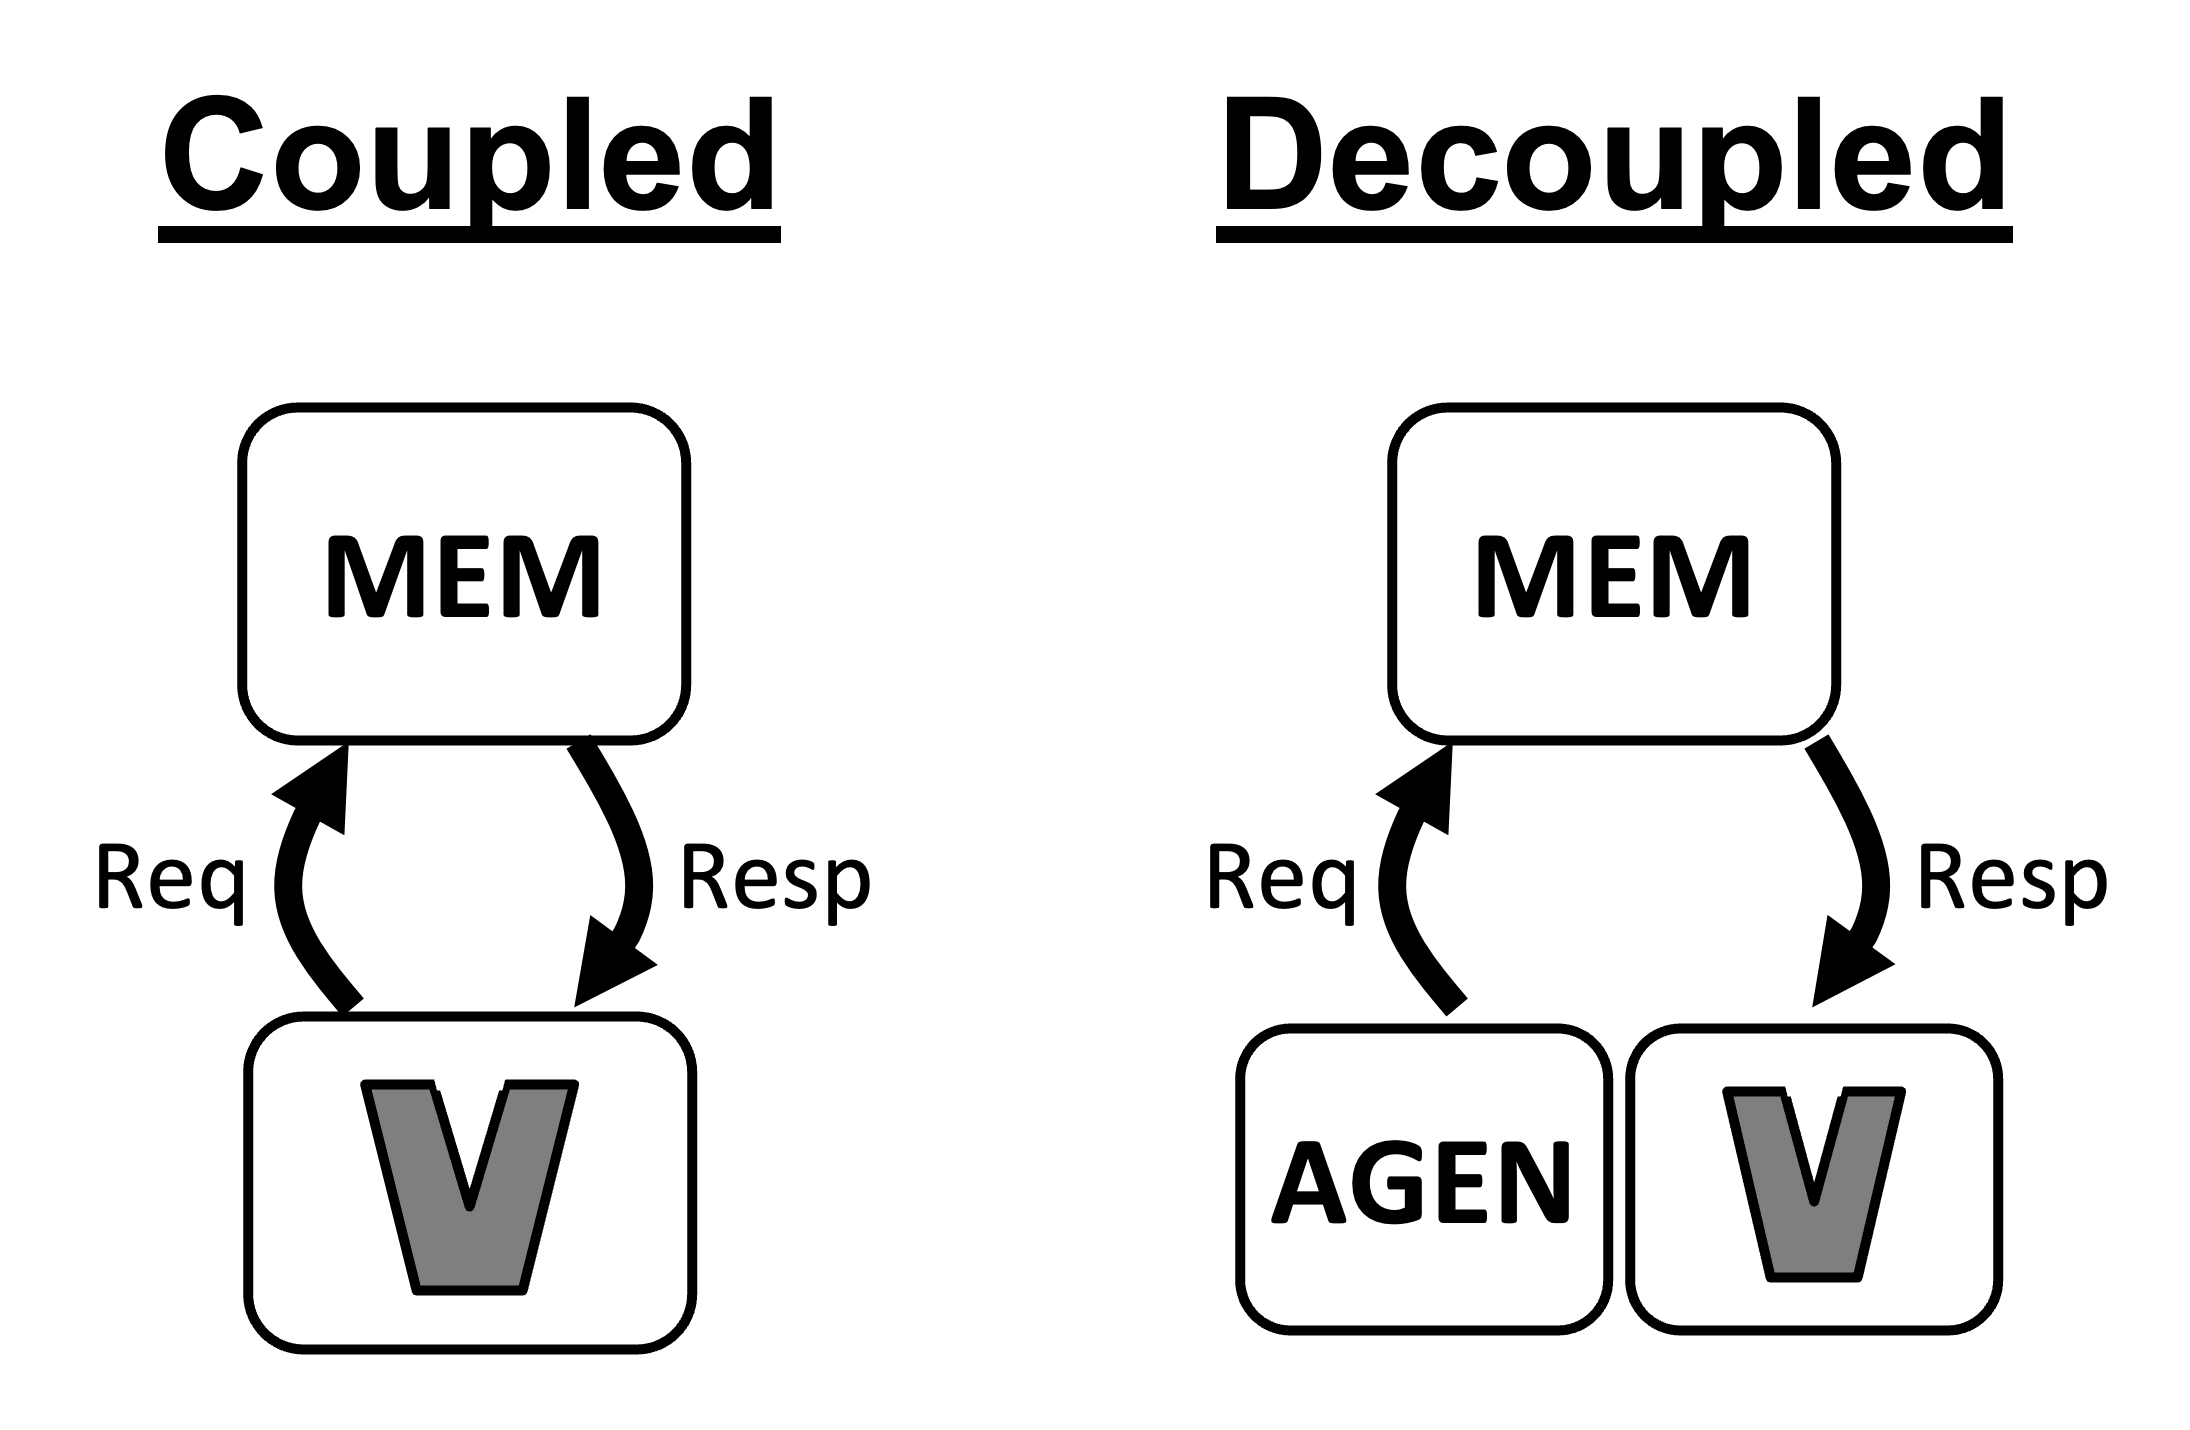
\includegraphics[width=0.5\textwidth]{figures/C_D_orchestration.png}
\caption{Data orchestration taxonomy from~\cite{buffet}. In \textit{Coupled} orchestration (\textit{left}) a module accesses data which it previously requested, while in \textit{decoupled} orchestration (\textit{right}) a separate \textit{address-generator} (AGEN) orchestrates data movement, anticipating a known deterministic pattern of future accesses by the module.}
\label{fig:C_D_orchestration}
\end{figure}

A ``taxonomy of data orchestration approaches'' for domain-specific hardware accelerators was proposed in~\cite{buffet}, and is partially reproduced and simplified in Figure~\ref{fig:C_D_orchestration}. In creating this taxonomy, the authors' intention was to (1) categorize common approaches to sequencing data movement within memory hierarchies, in order to (2) motivate an ``efficient and composable'' storage idiom (Buffets\cite{buffet}) optimized for a particular, desirable form of data orchestration known as \textit{Explicit Decoupled Data Orchestration} or EDDO. 

In the taxonomy of~\cite{buffet}, memories such as caches employ \textit{implicit} orchestration, because they hide complex and autonomous cache fill/eviction policies behind an interface that is indistinguishable from directly accessing memory, from the perspective of a downstream component. \textit{Explicit} orchestration refers to direct control of data movement within the memory hierarchy, based on direct commands that are conveyed via user programming or as part of requests issued by a downstream component. The explicit/implicit dichotomy will not be discussed further here, as it is less relevant to this work than the \textit{coupled/decoupled} dichotomy. This dichotomy refers to the way that memory access requests are handled. In a \textit{coupled} memory access paradigm, the component or module that is the ultimate consumer of some data stored in memory, is responsible for issuing requests to access that data. In contrast, a \textit{decoupled} memory access paradigm is possible in domain-specific accelerators which can anticipate a deterministic sequence of memory accesses. A component accesses memory assuming that the data it requires has already been filled and is resident at the appropriate level of the memory hierarchy. A separate (``decoupled'') component or module is responsible for overlapping each memory read with a request to fill new data into local memory; this requires that this sidecar component be pre-programmed with the deterministic sequence of memory accesses. Such a component is referred to as an \textit{address generator} (AGEN) in~\cite{buffet}. Figure~\ref{fig:C_D_orchestration} illustrates only the \textit{coupled}/\textit{decoupled} aspect of the taxonomy.

The authors of~\cite{buffet} note a number of benefits of an EDDO dataflow, such as lowering pressure on the memory system. The data orchestration taxonomy of \cite{buffet} is included here for three reasons: first, EDDO data orchestration is a baseline assumption by Timeloop\cite{timeloop}/Sparseloop\cite{sparseloop}, tools which this work will use as a starting-point for developing SAF microarchitecture modeling, (2) Section~\ref{chapter:conceptual_framework} will propose an EDDO buffer abstraction as an aid in decoupling SAF microarchitecture from dataflow, and (3) Section~\ref{chapter:conceptual_framework} further proposes that the degree of coupled memory access is a key distinction between SAF microarchitecture and non-SAF microarchitecture.

\section{Existing conceptual frameworks for sparse tensor accelerators}

This work builds on prior efforts to build conceptual frameworks around sparse tensor accelerators. All of the works in this section (except for Sparseloop\cite{sparseloop} itself) -  preceded Sparseloop, which introduced the term ``SAF''. Thus, any usage of the term ``SAF'' or ``SAF microarchitecture'' in this section is my own word choice and is not a quote.

\subsection{TACO\cite{taco}\cite{taco_format} hierarchical sparse tensor formats}
\label{sec:taco_format}

Building on the TACO tensor algebra compiler\cite{taco}, a unified abstraction for representing diverse sparse tensor representation formats was developed in \cite{taco_format} with the goal of providing general sparsity support in TACO\cite{taco}. Figure~\ref{fig:taco_format_example} illustrates the two of the many \textit{level format} data structures from \cite{taco_format}.

\begin{figure}[H]
\centering
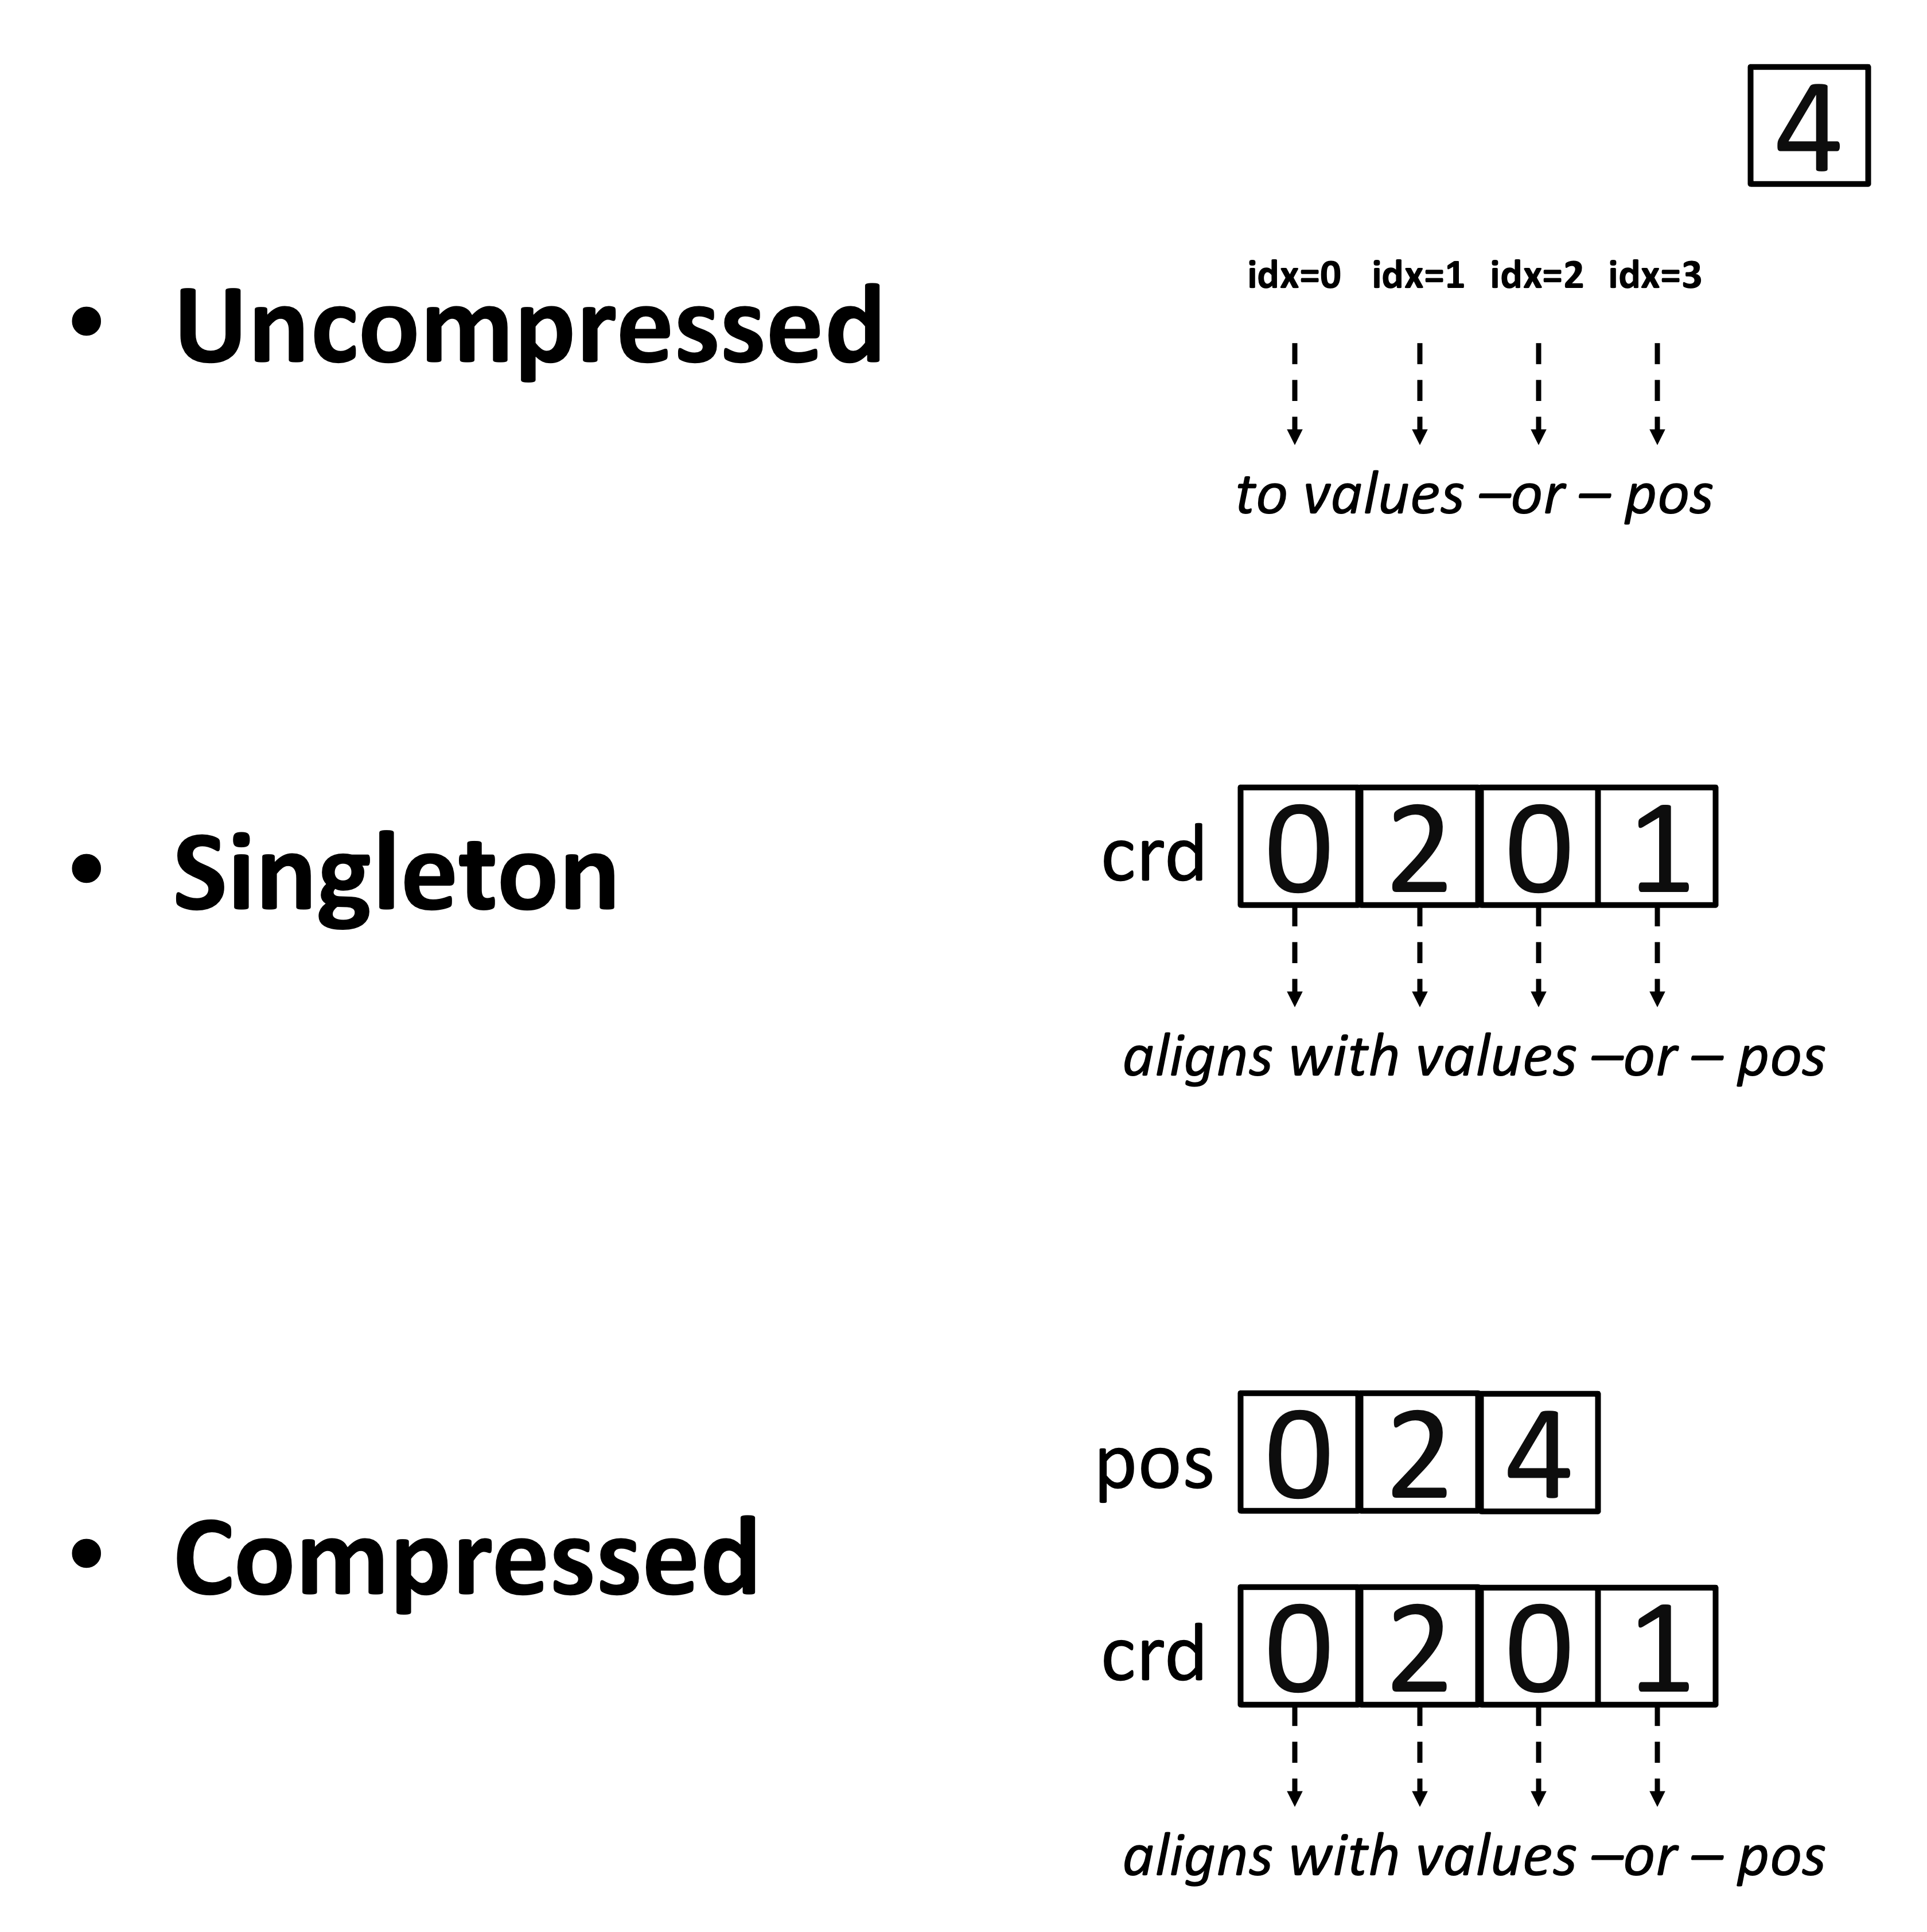
\includegraphics[width=0.5\textwidth]{figures/taco_levels.png}
\caption{A subset\cite{taco_format} of TACO\cite{taco} sparse \textit{level formats.}}
\label{fig:taco_levels}
\end{figure}

\cite{taco_format} proposes that many important sparse representation formats can be construed as tiered data structures in which each tier represents a tensor rank, represented using one of the handful of possible level formats. Figure~\ref{fig:taco_format_example} shows how compressed-sparse fiber (CSF)\cite{csf} and compressed-sparse row (CSR) can be represented within this unified sparse tensor abstraction.

\begin{figure}[H]
    \centering
    \begin{subfigure}[b]{0.4\textwidth}
        \centering
        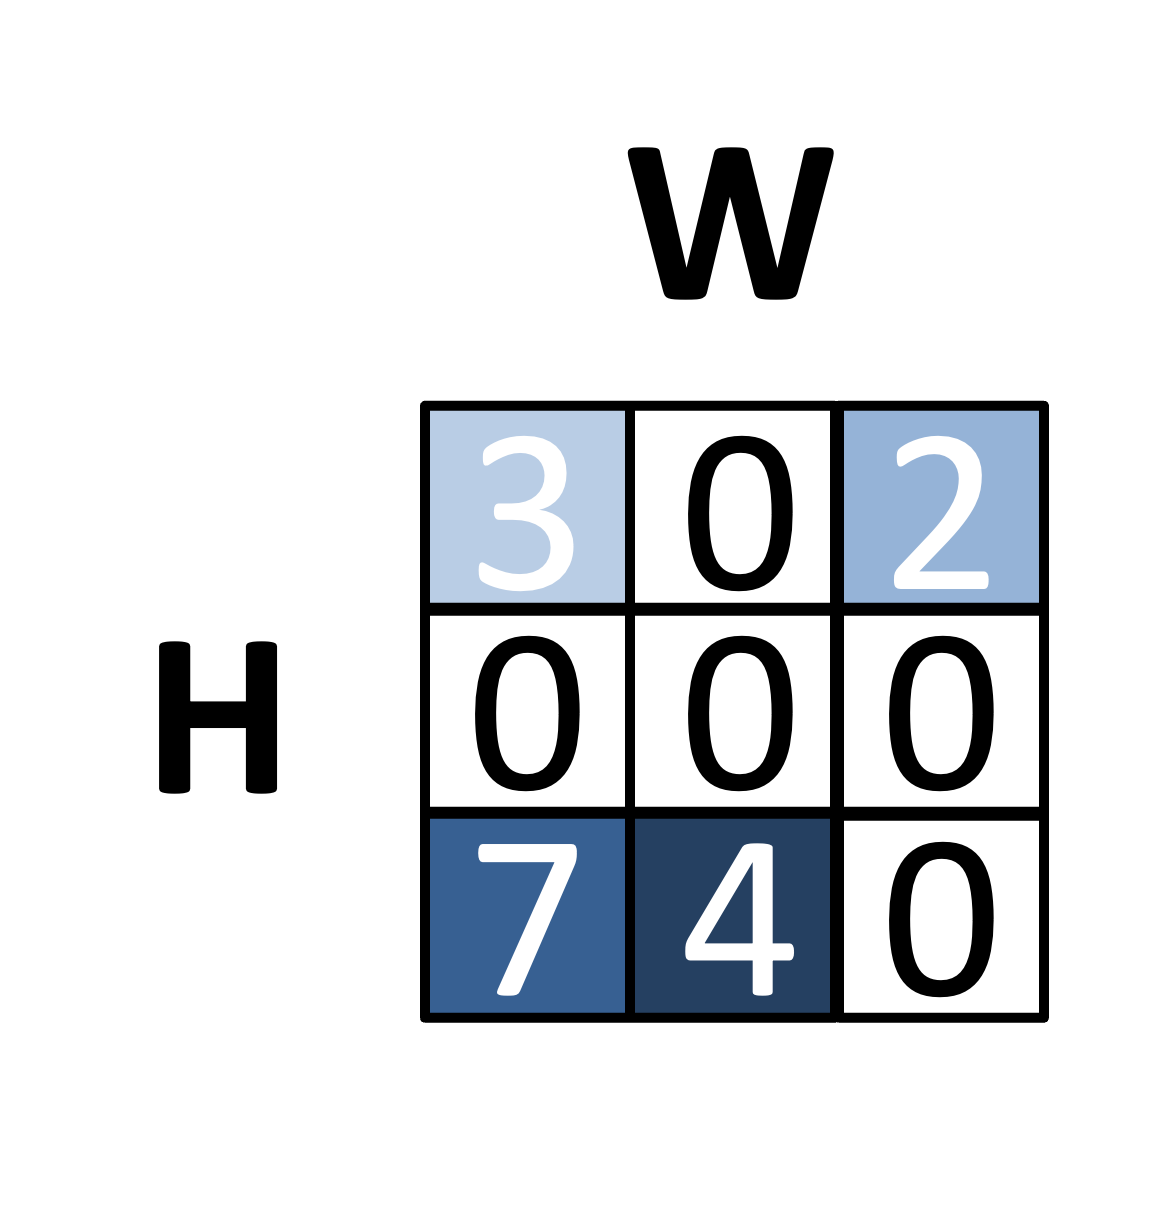
\includegraphics[width=\textwidth]{figures/taco_matrix.png}
        \caption{A 3x3 matrix.}
        \label{fig:taco_matrix}
    \end{subfigure}
    \hspace{0.5cm} % Adds space between the subfigures
    \begin{subfigure}[b]{0.4\textwidth}
        \centering
        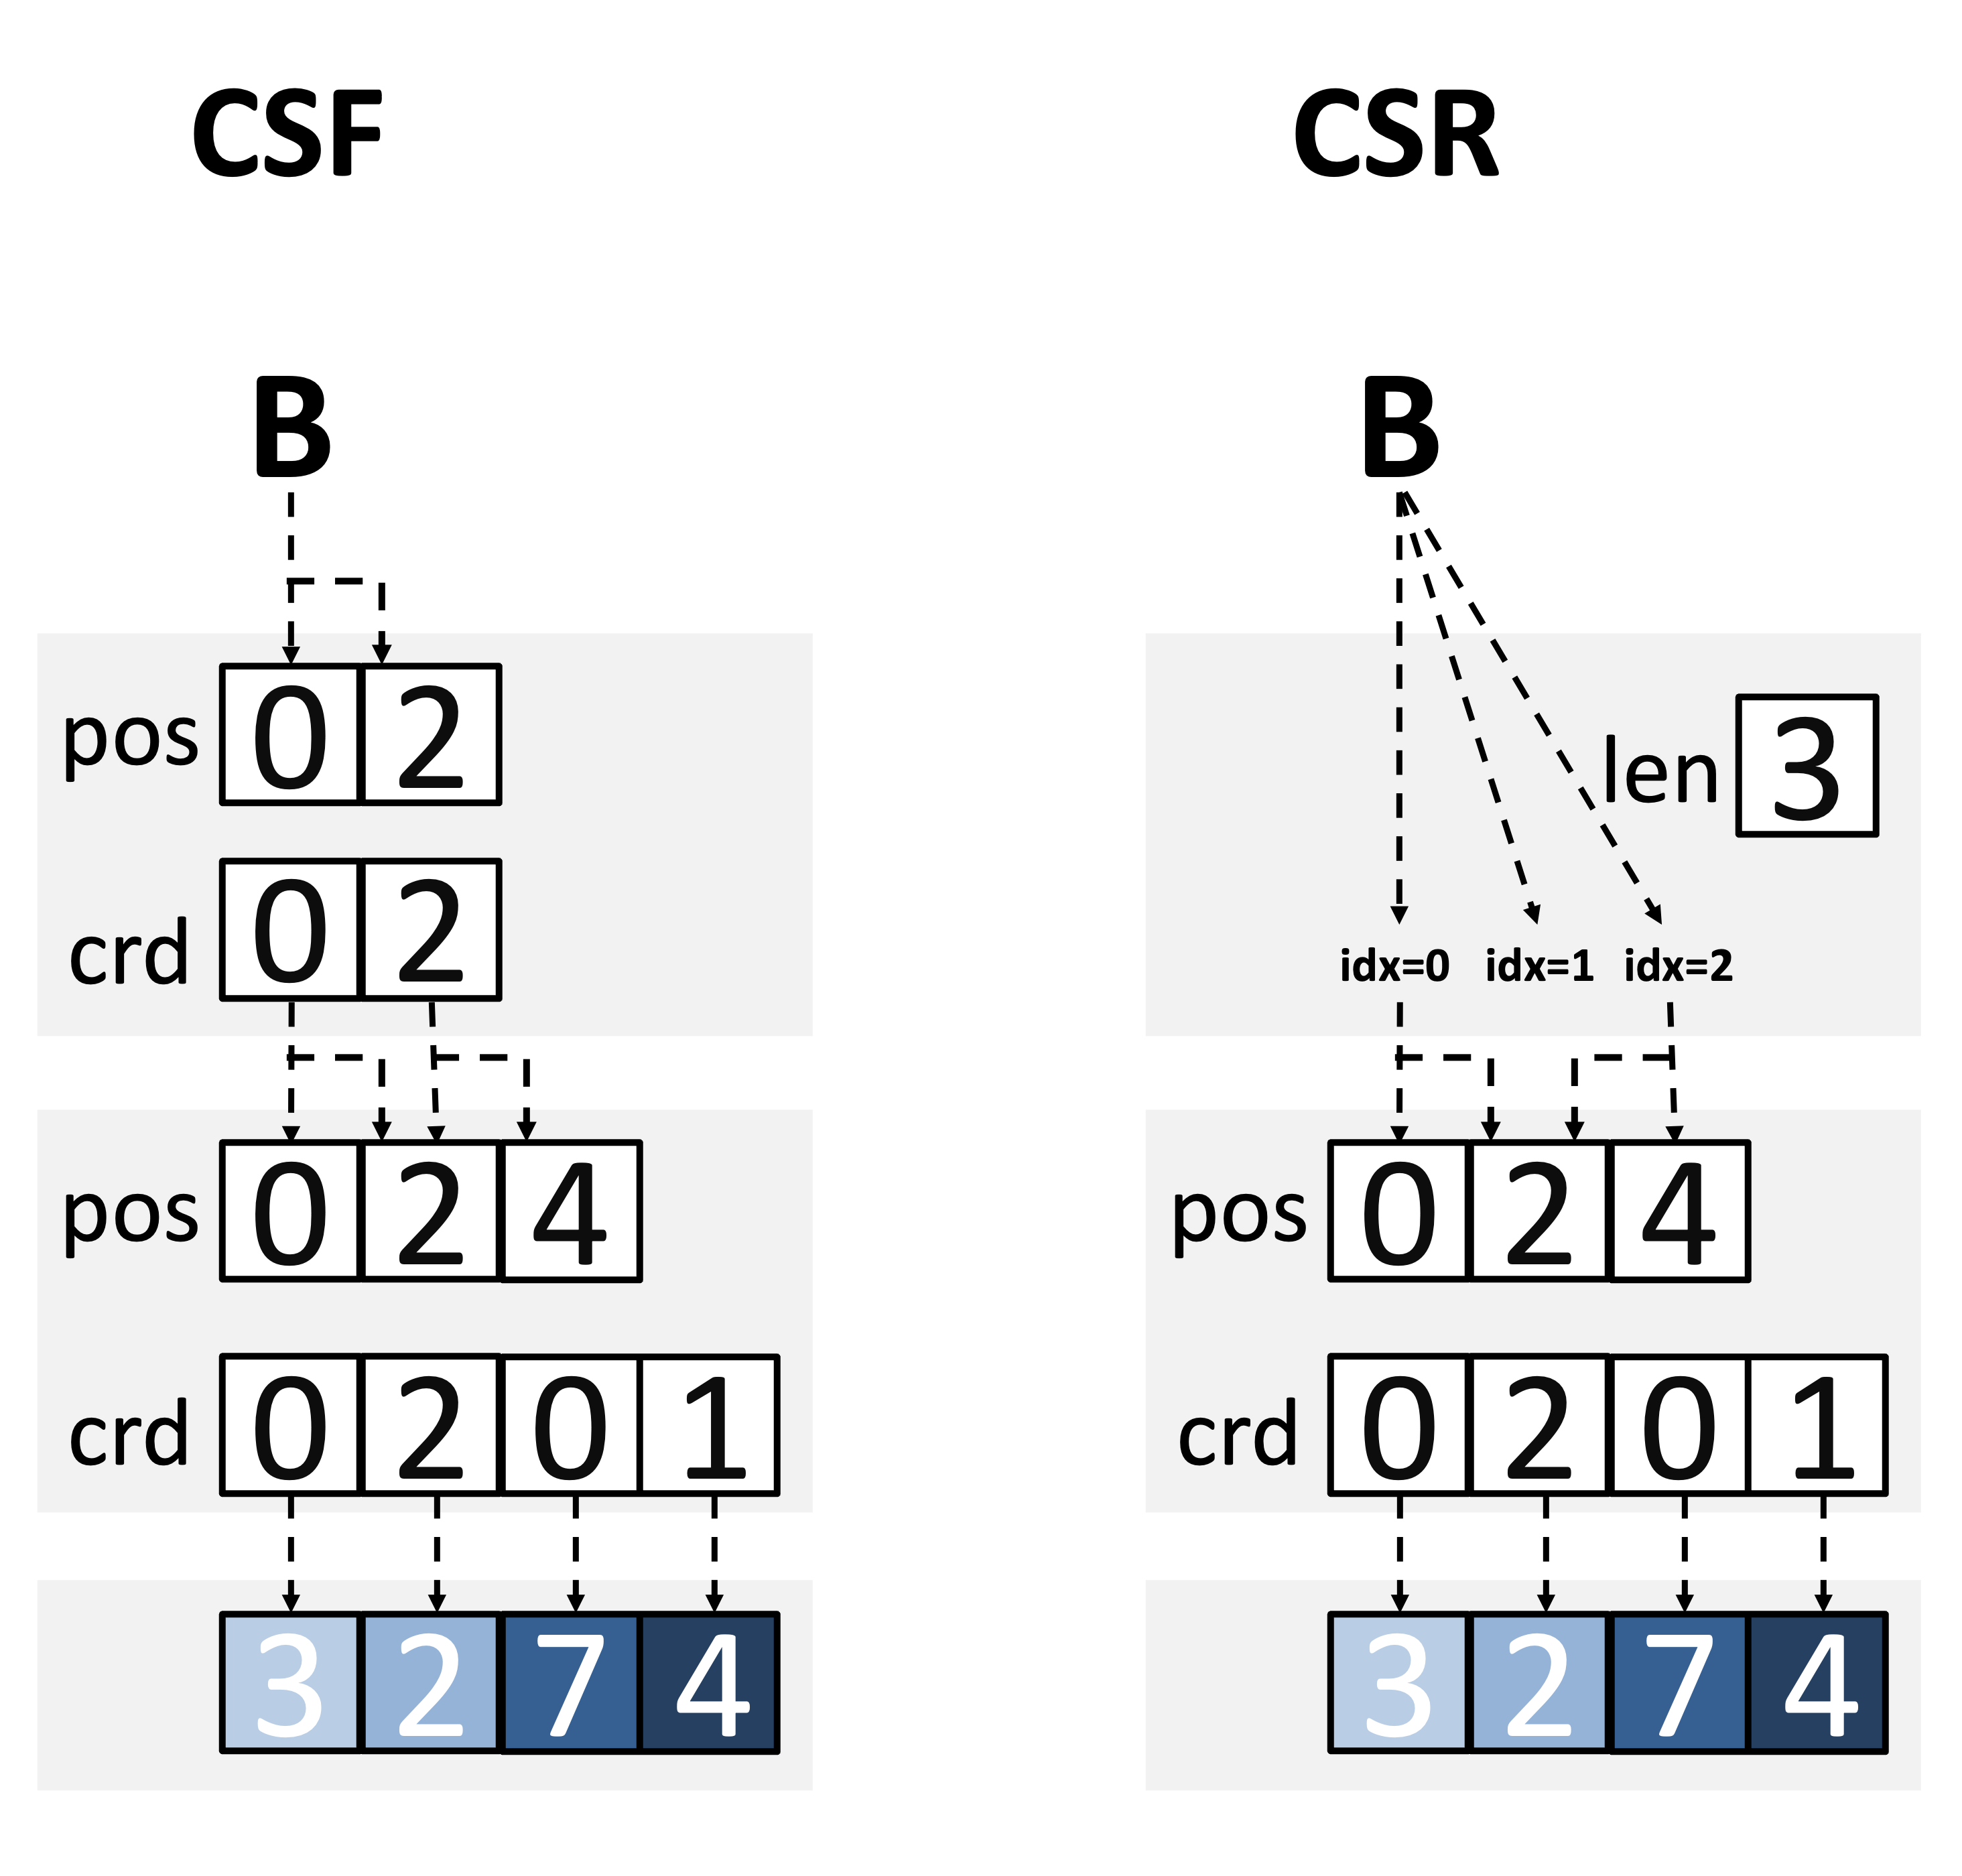
\includegraphics[width=\textwidth]{figures/taco_csf_csr.png}
        \caption{(\textit{left}) CSF\cite{csf} format, expressed with TACO\cite{taco} level formats and level abstraction\cite{taco_format} (\textit{right}) CSR format, again expressed with TACO levels and level abstraction. The matrix from Figure~\ref{fig:taco_matrix} is used as a reference.}
        \label{fig:taco_csf_csr}
    \end{subfigure}
    \caption{Example of representing a matrix (2nd-order tensor) in both CSF\cite{csf} and CSR formats, using level formats\cite{taco_format} and level hierarchy from the TACO\cite{taco} framework.}
    \label{fig:taco_format_example}
\end{figure}

To support compilation, level formats have a consistent programming model\cite{taco_format}. A level format supports certain \textit{capabilities} and certain \textit{properties}\cite{taco_format}, summarized in Table~\ref{tab:taco_capabilities_properties} for the two level formats in Figure~\ref{fig:taco_levels}.

\begin{table}[h]
\centering
\caption{An excerpt from Table 1 of the TACO sparse format paper\cite{taco_format} showing the abstract interface to each TACO level format. V: supports coordinate value iteration.  P: supports position iteration. I: supports insert. A: supports append. (\checkmark) indicates that the particular property is contingent on the fiber configuration, whereas a normal checkmark indicates full support.}
\resizebox{\textwidth}{!}{%
\begin{tabular}{|l|ccc|ccccc|}
\hline
\textbf{Level Type} & \multicolumn{3}{c|}{\textbf{Capabilities}} & \multicolumn{5}{c|}{\textbf{Properties}} \\ 
& \textbf{Iteration} & \textbf{Locate} & \textbf{Assembly} & \textbf{Full} & \textbf{Ordered} & \textbf{Unique} & \textbf{Branchless} & \textbf{Compact} \\
\hline
Uncompressed      & V & \checkmark & I & \checkmark & (\checkmark) & (\checkmark) & & \checkmark \\
Compressed & P & & A & (\checkmark) & (\checkmark) & (\checkmark) & & \checkmark \\
\hline
\end{tabular}
}
\label{tab:taco_capabilities_properties}
\end{table}

TACO level format capabilities comprise

\begin{itemize}
    \item \textbf{Iteration -} A set of methods for traversing a sparse tensor rank with the specified level format.
    \begin{itemize}
        \item \textbf{Value iteration -} Iterate through dense coordinates (not supported by the Compressed level format.)
        \item \textbf{Position iteration -} Iterate through elements which have entries in the \textit{pos} data structure.
    \end{itemize}
    \item \textbf{Locate -} Random-access lookup into a ``coordinate hierarchy level''. Lookup is by coordinate-value.
    \item \textbf{Assembly -} Additional capabilities for adding new coordinates to a level.
    \begin{itemize}
        \item \textbf{Insert -} Random-access insert a coordinate into some level at specified \textit{position.}
        \item \textbf{Append -} Append a coordinate at the end of a level.
    \end{itemize}
\end{itemize}

TACO level format properties comprise

\begin{itemize}
    \item \textbf{Full -} Among coordinates sharing the same ancestor at a given level, all coordinates are explicitly represented (counterexample: a compressed level format.)
    \item \textbf{Ordered -} Among coordinates sharing the same ancestor at a given level, coordinates are in sorted increasing order.
    \item \textbf{Unique -} Among coordinates sharing the same ancestor at a given level, every coordinate is encoded at most once (counterexample: COO.)
    \item \textbf{Branchless -} No coordinates have siblings and every coordinate in the previous level has a child.
    \item \textbf{Compact -} There are no empty encodings in the level representation - ``no coordinates are separated by an unlabeled node that does not encode a coordinate''\cite{taco_format}
\end{itemize}

\subsection{\textit{Efficient Processing}}

\textit{Efficient Processing of Deep Neural Networks}\cite{szebook} (Sze, Chen, et. al. 2020) (\textit{Efficient Processing} for short) introduced a number of abstractions for representing tensors in memory, for compressing tensor ranks, and for representing sparse dataflows. In practice the latter is closest to an existing taxonomy of SAF microarchitecture. 

\subsubsection{\textit{Efficient Processing} fibertree abstraction}

Building on \cite{taco_format} (Section~\ref{sec:taco_format}) as well as \cite{extensor}, the authors of \textit{Efficient Processing} proposed a TACO-like hierarchical representation of sparse tensors, called the ``fibertree'' abstraction (Figure~\ref{fig:efficient_processing_fibertree}.) The TACO level format abstraction was motivated by avoiding the need to hard-code a new data structure and new sparse dataflow for each new representation format TACO supports\cite{taco_format}; the \textit{Efficient Processing} fibertree abstraction is motivated by a desire to decouple sparse representation format from sparse dataflow for hardware engineers in the early stages of design and planning\cite{szebook}. As with TACO\cite{taco_format}, \textit{Efficient Processing} defines a set of possible sparse representation formats, and then builds a framework for composing them into sparse tensor representation formats.

\subsubsection{\textit{Efficient Processing} taxonomy of sparse representation formats}

\textit{Efficient Processing}\cite{szebook} introduced a taxonomy of sparse representation formats. We will not discuss the \textit{Efficient Processing} taxonomy at length here, choosing for brevity to instead focus on the taxonomy of sparse representation formats introduced in the Sparseloop\cite{sparseloop} paper which will be introduced later. However, \textit{Efficient Processing} introduced the concepts of \textit{explicit and implicit representation formats} which are relevant in this work.

\paragraph{Explicit and implicit representation formats.} \textit{Efficient Processing} categorizes sparse representation formats based on whether they have \textit{explicit coordinates} - i.e. the compressed payloads are associated with metadata that calls out specified coordinate values - or \textit{implicit coordinates} - i.e. the compressed payloads are associated with a metadata data structure which encodes coordinates but does not represent them explicitly.

In this work, implicit representation formats such as bitmask will entail increased overhead owing to the need to recover explicit coordinates in certain situations.
%\begin{figure}[H]
%\includegraphics[width=\textwidth]{figures/representat}
%\caption{An example of the \textit{Efficient Processing} fibertree abstraction, applied to the matrix in Figure~\ref{fig:taco_matrix}.}
%\label{fig:efficient_processing_fibertree}
%\end{figure}

\subsubsection{Fibertrees}
\label{sec:fibertrees}

\begin{figure}[H]
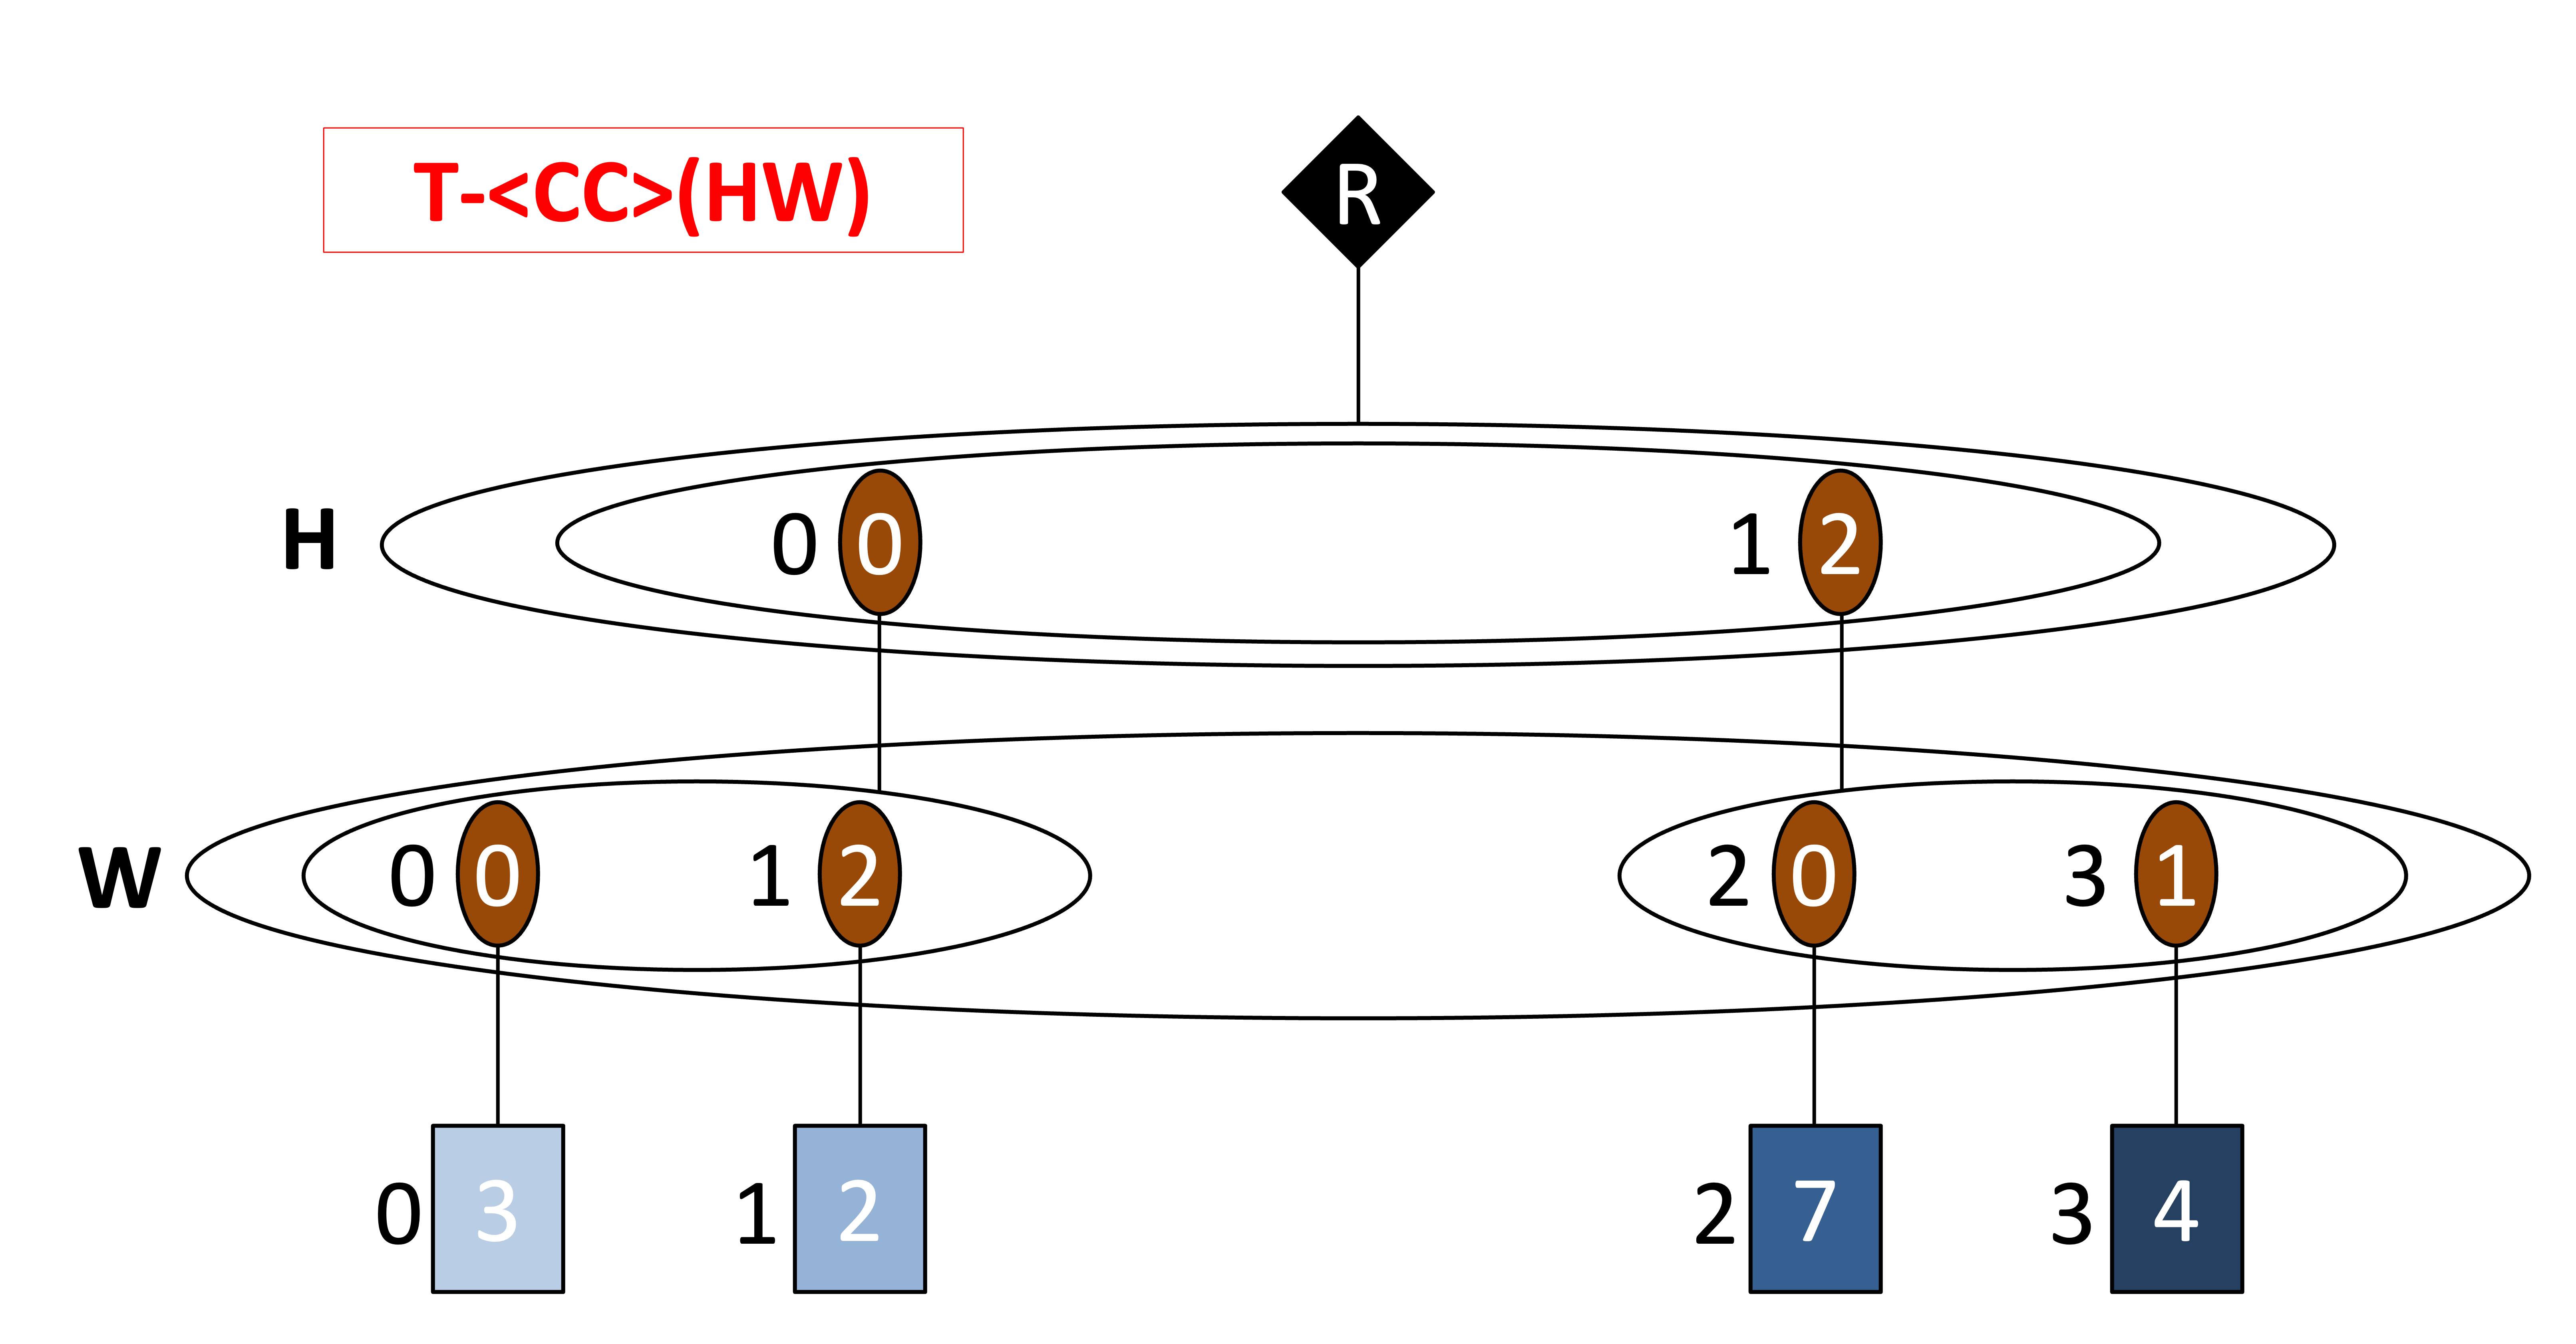
\includegraphics[width=\textwidth]{figures/efficient_processing_fibertree.png}
\caption{An example of the \textit{Efficient Processing} fibertree abstraction, applied to the matrix in Figure~\ref{fig:taco_matrix}.}
\label{fig:efficient_processing_fibertree}
\end{figure}

As with the TACO framework for describing sparse representation formats, a fibertree is a tiered structure assembled by composing named levels - \textit{ranks}. As with the CSF format\cite{csf}, each rank represents a tensor axis. A rank contains multiple \textit{fibers}, and each fiber is an sort-ordered list of coordinates which is itself the child of a coordinate in the next higher rank; each coordinate has a child - a \textit{payload} - which is either a fiber in the next lower rank, or the value of an element in the tensor. Unlike the TACO framework, fibertree ranks abstract away the details of memory layout that are discussed in \cite{taco_format}.

\paragraph{Parts of a fibertree.}

\begin{itemize}
    \item \textbf{Rank:} A representation of a tensor axis, assigned a name \textit{rank-id}.
    \item \textbf{Coordinate:} A numeric identifier associated each element or item in a rank.
    \item \textbf{Payload:} The ``value'' associated with a given coordinate in a fiber. Only the lowest rank of a fibertree associates coordinates with payloads which are singleton data values; otherwise, payloads of a coordinate in a given rank are actually \textit{sub-trees} rooted at the given coordinate.
    \item \textbf{Point:} The set of coordinates which represent a path from the root of the tensor to the element of interest
\end{itemize}

\paragraph{Tensor notation.} \textit{Efficient Processing} introduced \textit{tensor representation notation}\cite{szebook} for concisely describing a fibertree in terms of its sequence of rank formats, from top to bottom in the fibertree:

Tensor-<\textbf{FIBER-REPRESENTATION-REGEX}>(RANK-ID...)

or more concisely,

T-<\textbf{FIBER-REPRESENTATION-REGEX}>(RANK-ID...)

where

\begin{itemize}
    \item \textbf{FIBER-REPRESENTATION-REGEX} is a list of sparse representation format abbreviations which matches the rank formats in the fibertree, from top to bottom.
    \item \textbf{RANK-ID} is a list of rank names, from top to bottom in the fibertree.
\end{itemize}

So for example, describing the fibertree in Figure~\ref{fig:efficient_processing_fibertree} as T-<CC>(HW) means that it has two ranks, named \textbf{H} and \textbf{W}, which are both in coordinate payload (C) format.

\subsubsection{\textit{Efficient Processing} Sparse dataflow \& SAF microarchitecture primitives}

Section 8.3 of \textit{Efficient Processing} introduced a framework for implementing ``sparse architecture dataflows''. The principle of this framework is that (1) the choice of sparse representation format frequently must be co-designed with SAF microarchitecture, however (2) it will be simpler to talk about sparse representation formats or SAF microarchitectures, respectively, if they each have decoupled representations; then co-design becomes effectively the cartesian product of possible sparse architectures and possible sparse format representations. 

Section 8.2 of \textit{Efficient Processing} already introduced fibertrees as a simple and intuitive abstraction for sparse representation formats, decoupled from the underlying microarchitecture. To that end, Section 8.3 of \textit{Efficient Processing} introduces two different abstractions for representing a sparse architecture dataflow which are decoupled from specific sparse representation formats:

\begin{itemize}
    \item \textbf{Dataflow as a loop nest.} Timeloop\cite{timeloop} represents dense architecture dataflows as loop nests which iterate \textit{by index} over coordinate values. \textit{Efficient Processing} introduces sparse loop nests, which extend Timeloop loop nest pseudocode with TACO\cite{taco_format}-style position iteration: each loop iteration uses Pythonic iterate-by-value syntax to get the next $(coord,pos)$ pair.
    \item \textbf{Dataflow as a topology built from a component taxonomy.} Once a sparse architecture dataflow is represented as a sparse loop nest, the aim of the \textit{Efficient Processing} framework is that this loop nest can be intuitively transformed to a microarchitecture topology. Based on the principle of decoupling format from dataflow, Section 8.3.1 of \textit{Efficient Processing} introduces a taxonomy of format-agnositic microarchitecture primitives. Each primitive is a either a memory, a sequence generator, a microarchitecture for comparing sparse format metadata streams, or some form of arithmetic. Each primitive has a set of ports associated with some datatype. These primitives are wired together into a topology which is animated by sequences of positions or coordinates from the sequence generators, thus implementing the sparse architecture dataflow.
\end{itemize}

\begin{figure}[H]
    \centering
    \begin{subfigure}[b]{0.2\textwidth}
        \centering
        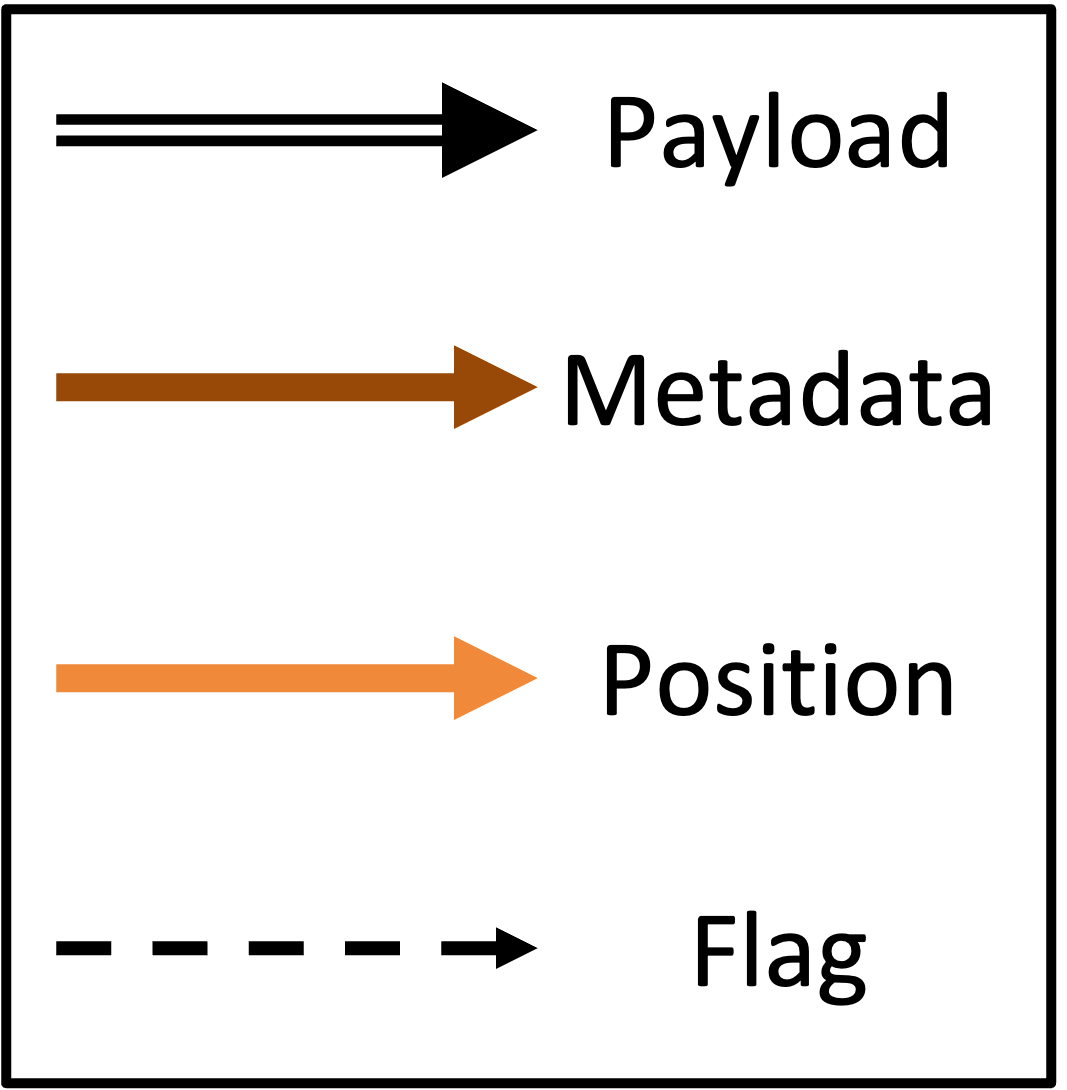
\includegraphics[width=\textwidth]{figures/efficient_processing_wire_legend.png}
        \caption{Wire types in the \textit{Efficient Processing} structural taxonomy for sparse architecture dataflows.}
        \label{fig:efficient_processing_wire_legend}
    \end{subfigure}
    \vspace{1cm} % Adds space between the subfigures
    \begin{subfigure}[b]{0.95\textwidth}
        \centering
        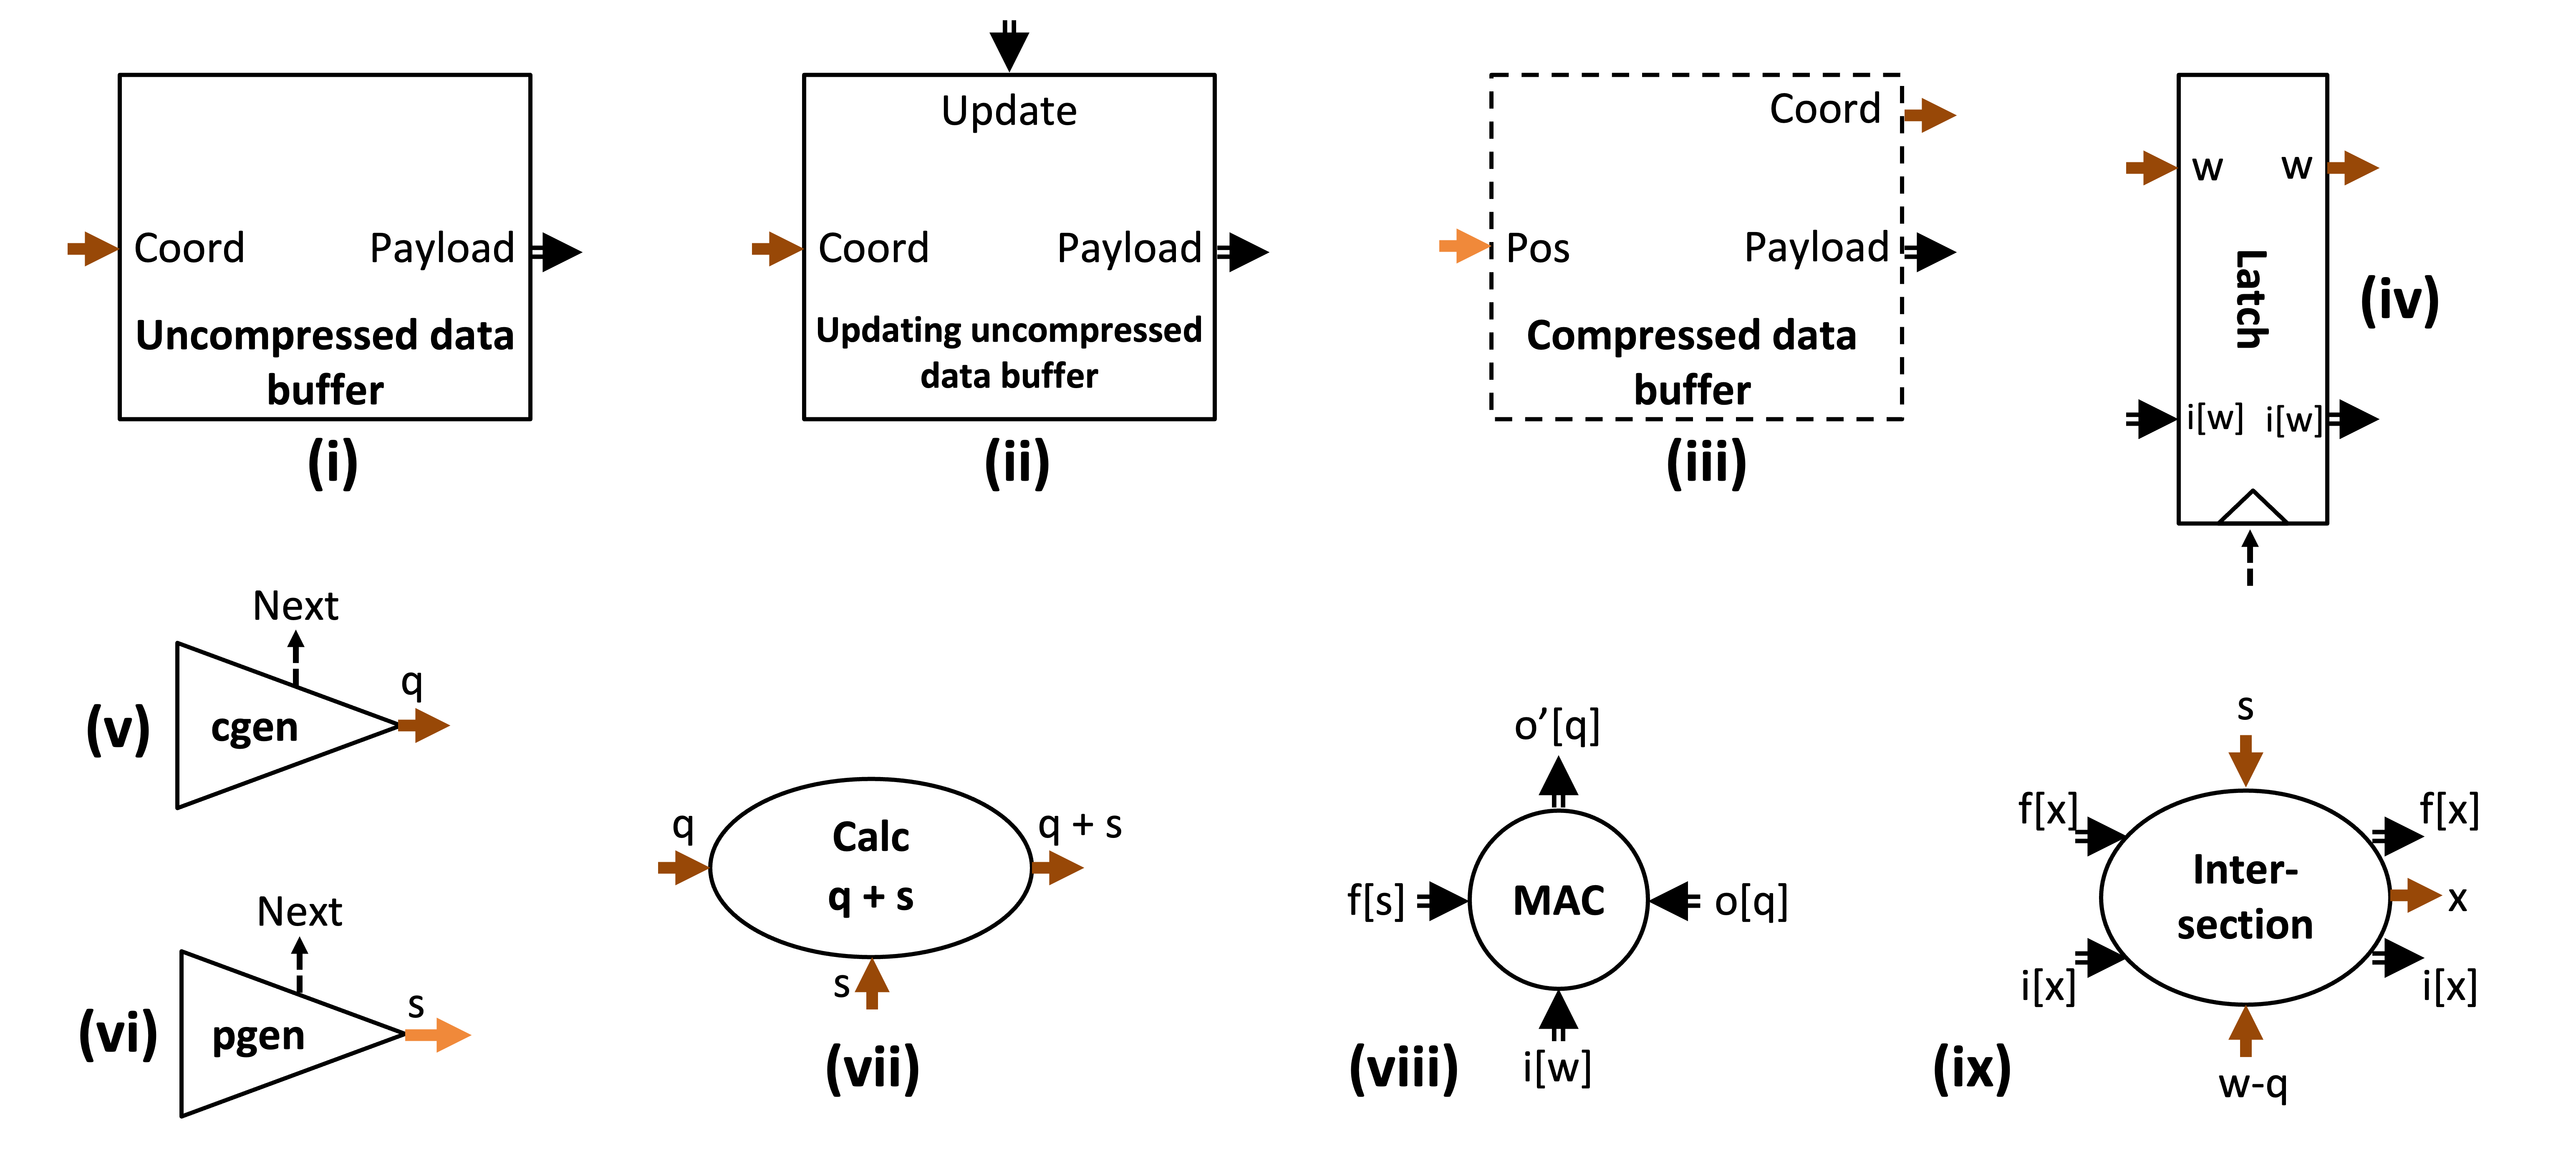
\includegraphics[width=\textwidth]{figures/efficient_processing_taxo.png}
        \caption{Components in the \textit{Efficient Processing} structural taxonomy for sparse architecture dataflows.}
        \label{fig:efficient_processing_taxo}
    \end{subfigure}
    \caption{Combined figure of wire types and components in the \textit{Efficient Processing} structural taxonomy.}
\end{figure}

Figure~\ref{fig:efficient_processing_wire_legend} and Figure~\ref{fig:efficient_processing_taxo} summarize the framework for building microarchitecture topologies. In this domain-specific framework, there are four types of wires (Figure~\ref{fig:efficient_processing_wire_legend}):

\begin{itemize}
    \item \textbf{Payload (black double-line) -} the data referenced by metadata; may comprise sub-tiles or individual data elements depending on the context of the larger design.
    \item \textbf{Metadata (brown single-line) -} a stream of sparse format metadata words.
    \item \textbf{Position (yellow-orange single-line) -} a stream of address offsets into architectural buffer memory (as distinct from coordinates which are offsets into dense coordinate space, and which are usually represented by brown metadata wires.)
    \item \textbf{Flag (dashed black line) -} a one-bit control signal, usually employed to synchronize control signals between components.
\end{itemize}

These are also the four possible port datatypes. There are nine primitives in this framework (Figure~\ref{fig:dense_smartbuffer_composition}):

\begin{itemize}
    \item \textbf{(i) Uncompressed data buffer -} a buffer with no sparse format optimization. Payloads are read by directly specifying coordinates as lookup addresses, which is possible because coordinates and positions are the same in a dense data structure. 
    \item \textbf{(ii) Updating uncompressed data buffer -} represents a buffer with support for both read and write (update) operations, and no format optimization.
    \item \textbf{(iii) Compressed data buffer - } a buffer with a sparse format representation. A payload and its associated memory data are selected by a positional input.
    \item \textbf{(iv) Latch - } Single architectural register for holding a datatype stationary.
    \item \textbf{(v) Coordinate generator - } Sequence generator for abstract coordinates.
    \item \textbf{(vi) Position generator - } Sequence generator for address offsets in memory.
    \item \textbf{(vii) Coordinate calculator - } small, low-cost arithmetic unit which is required to implement the projection expressed by the problem dataspace.
    \item \textbf{(viii) Multiply Accumulate Unit (MAC) - } Compute.
    \item \textbf{(ix) Intersection unit - } Stand-in for a variety of components which select pairs of operand payloads based on an inner join on coordinate metadata.
\end{itemize}

As a way of illustrating different sparse dataflows, Section 8.3 of \textit{Efficient Processing} expresses a number of contemporary sparse tensor accelerator designs (\cite{cambricon_x}\cite{cnvlutin}\cite{scnn}\cite{sparten}\cite{eyerissv2}\cite{eie}\cite{extensor}), first in sparse loop nest form, and then as microarchitecture topologies which implement the sparse loop nests.

% \subsection{Sparse abstract machine}

\subsection{Sparseloop}

Section~\ref{chapter:introduction} briefly introduced Accelergy\cite{accelergy}, Timeloop\cite{timeloop}, and Sparseloop\cite{sparseloop}. Put briefly -

\begin{itemize}
    \item Accelergy\cite{accelergy} is a framework for pre-RTL analytical modeling of hardware components. Conceptually, the authors of Accelergy propose a framework in which (1) the cost of a component is modeled as an area value, as well as a set of energy values associated with specific actions (``energy-per-action'') defined by the modeling engineer, (2) reuse of models is maximized through support for \textit{compound component} models which derive area and energy-per-action from the composition of multiple \textit{primitive components}, and (3) component models are parameterized, allowing the modeling engineer to scale a component's bitwidth, number of memory banks, etc. in order to support the workload that is being modeled. Practically, the Accelergy framework is surfaced to users as a CLI tool for evaluated area and energy per action, given a model description or description(s) and associated model parameters.
    \item Timeloop\cite{timeloop} is a framework for fast analytical modeling of \textit{dense} tensor accelerators. ``Fast analytical modeling'' is positioned in contrast to (1) cycle-accurate simulation, which may be time-consuming, and (2) layout-level simulation modeling, which is almost always very-consuming\cite{wattch}. Timeloop is capable of modeling architectural energy, area, memory footprint, and memory accesses, as well as dataflow\cite{timeloop}; Timeloop is intended to support early-stage design-space exploration and trade-off decisions by ASIC architects, long before the accelerator is actually implemented.
\end{itemize}

Sparseloop\cite{sparseloop} extends Timeloop with support for Sparsity. Sparseloop developed a unified taxonomy of Sparse Acceleration Features (SAFs), architectural optimization strategies for exploiting sparsity (zero-sparsity) to conserve energy and cycles. A SAF is a strictly declarative description of an optimization, comprising (1) a description of the optimization outcome (i.e. skipping of certain compute operatinos), (2) a set of attributes which modulate the outcome of the optimization, and (3) a binding to a particular architectural buffer or compute component. A SAF describes neither the microarchitectural implementation of the optimization, nor the interfaces or communication protocols involved in integrating the microarchitectural implementation into the design. 

Nonetheless, a real design would require a microarchitectural change which implements the optimization, referred to here as the \textit{SAF microarchitecture.} Existing analytical modeling tools\cite{sparseloop} model only the benefits of exploiting SAFs (savings on memory capacity, fewer memory accesses, fewer compute cycles); these benefits are introduced in Section~\ref{background:safs}. These tools avoid modeling the costs of SAF microarchitectures by assuming (1) an ideal SAF microarchitecture which perfectly implements the SAF, and (2) a SAF microarchitecture with negligible energy and area overhead.

This section introduces the set of sparse representation formats considered in the Sparseloop paper, as well as the Sparseloop unifed SAF taxonomy. Subsequently, Section~\ref{background:saf_uarch} demonstrates that SAF microarchitectures can \textit{sometimes} have significant implications for the design and modeling of sparse tensor accelerators. Thus, this work is motivated by the need to create novel SAF microarchitecture models.

\subsubsection{Sparse representation formats}
\label{background:sparseloop_formats}

The three sparse representation formats studied in Sparseloop\cite{sparseloop} are

\begin{itemize}
    \item \textbf{Uncompressed (U)} - a vector as it exists in memory without any compression, including zero-value elements.
    \item \textbf{Uncompressed Offset Pairs (UOP)} - An uncompressed fiber format in which the payloads are ranges of offsets into another rank (this is discussed in Section~\ref{sec:fibertrees}.)
    \item \textbf{Coordinate Payload (C)} - A compressed fiber format comprising an array of non-zero payloads, each with a corresponding explicit coordinate value.
    \item \textbf{Bitmask (B)} - A compressed fiber format comprising an array of non-zero payloads, and a metadata array which is a bitmask of length equal to the size of the underlying uncompressed rank. The indices of non-zero entries (hot bits) in the metadata bitmask are the coordinates of corresponding non-zero payloads.
\end{itemize}

%
% SAFs subsection
%
\subsubsection{SAFs}
\label{background:safs}

This section will review and motivate the two broad SAF categories, format and action SAFs.

%
% Figure: examples of action optimizations
%
%\begin{figure}[H]
%\includegraphics[width=\textwidth]{figures/saf_action_optimizations.PNG}
%\caption{An example of dot-product optimized with zero-gating and zero-skipping to save cycles and energy, versus the naive un-optimized approach. The zero-skipping optimization's efficacy may depend on the choice of leader-follower skipping vs bidirectional skipping.}
%\label{fig:saf_action_optimizations}
%\end{figure}
%
% Table: Action SAFs, comparison of perf and energy
%
%\begin{table}[ht]
%\begin{tabular}{c|c|c|}
% & Cycles & Energy \\ \hline \hline
%Theoretical &  \textcolor{green}{\textbf{1}} & \textcolor{green}{\textbf{$E_{mac}$}}\\ \hline
%Naive &  \textcolor{red}{\textbf{5}} & \textcolor{red}{\textbf{$5 E_{mac}$}}\\ \hline
%Zero-gating &  \textcolor{red}{\textbf{5}} & \textcolor{green}{\textbf{$E_{mac}$}} \\ \hline
%Zero-skipping (leader-follower) & \textcolor{red}{\textbf{2}} & \textcolor{red}{\textbf{$2 E_{mac}$}} \\ \hline
%Zero-skipping (bidirectional) & \textcolor{green}{\textbf{1}} & \textcolor{green}{\textbf{$E_{mac}$}} \\ \hline
%\end{tabular}
%\caption{Dot-product cycles and energy with different action-optimization strategies applied to the PE in Figure \ref{fig:saf_action_optimizations}, versus the theoretical-best. Energy is measured in multiples of the energy of a single MAC, $E_{mac}$}
%\label{tab:action_saf_comparison}
%\centering
%\end{table}
%
% Content: SAFs
%
\paragraph{Action optimizations.} These are SAFs which signify that the tensor accelerator detects and optimizes away ineffectual operations such as $0 \times 0 = 0$ and $0 \times a = 0$, with the goal of saving energy and potentially compute cycles. Gating SAFs save on the energy associated wth IneffOps\cite{sparseloop}, by quiescing relevant components during the cycle when the operation occurs. Skipping SAFs save on energy \textit{and} cycles, by bypassing the IneffOp entirely and jumping ahead to the next operation.

Designs with \textit{bidirectional action optimizations} skip or gate when either operand is zero. Thus 100\% of gating or skipping opportunities are exploited, depending on the type of action optimization. Designs with \textit{leader-follower action optimizations} respond only to the designated leader operand being zero, in which case both the MAC and the follower memory access are skipped or gated; ineffectual follower operands incur no savings.

Thus, the key attribute for both skipping and gating action optimizations is direction (\textit{bidirectional} vs \textit{leader-follower}, and also the particular architectural element (buffer or arithmetic) which the SAF is bound to.

%
\paragraph{Format optimizations.} The zero-compression (or \textit{format}) SAF discards ineffectual zero-valued tensor elements in order to save memory capacity at rest and memory bandwidth during accesses\cite{sparseloop}. The remaining nonzero values' positions in memory no longer align with the original coordinates, so the compressed format requires metadata which may be used to recover an element's uncompressed coordinate as efficiently as possible.

These are derived from the Sparseloop\cite{sparseloop} paper.

%
% Figure: examples of format optimizations
%
%\begin{figure}[H]
%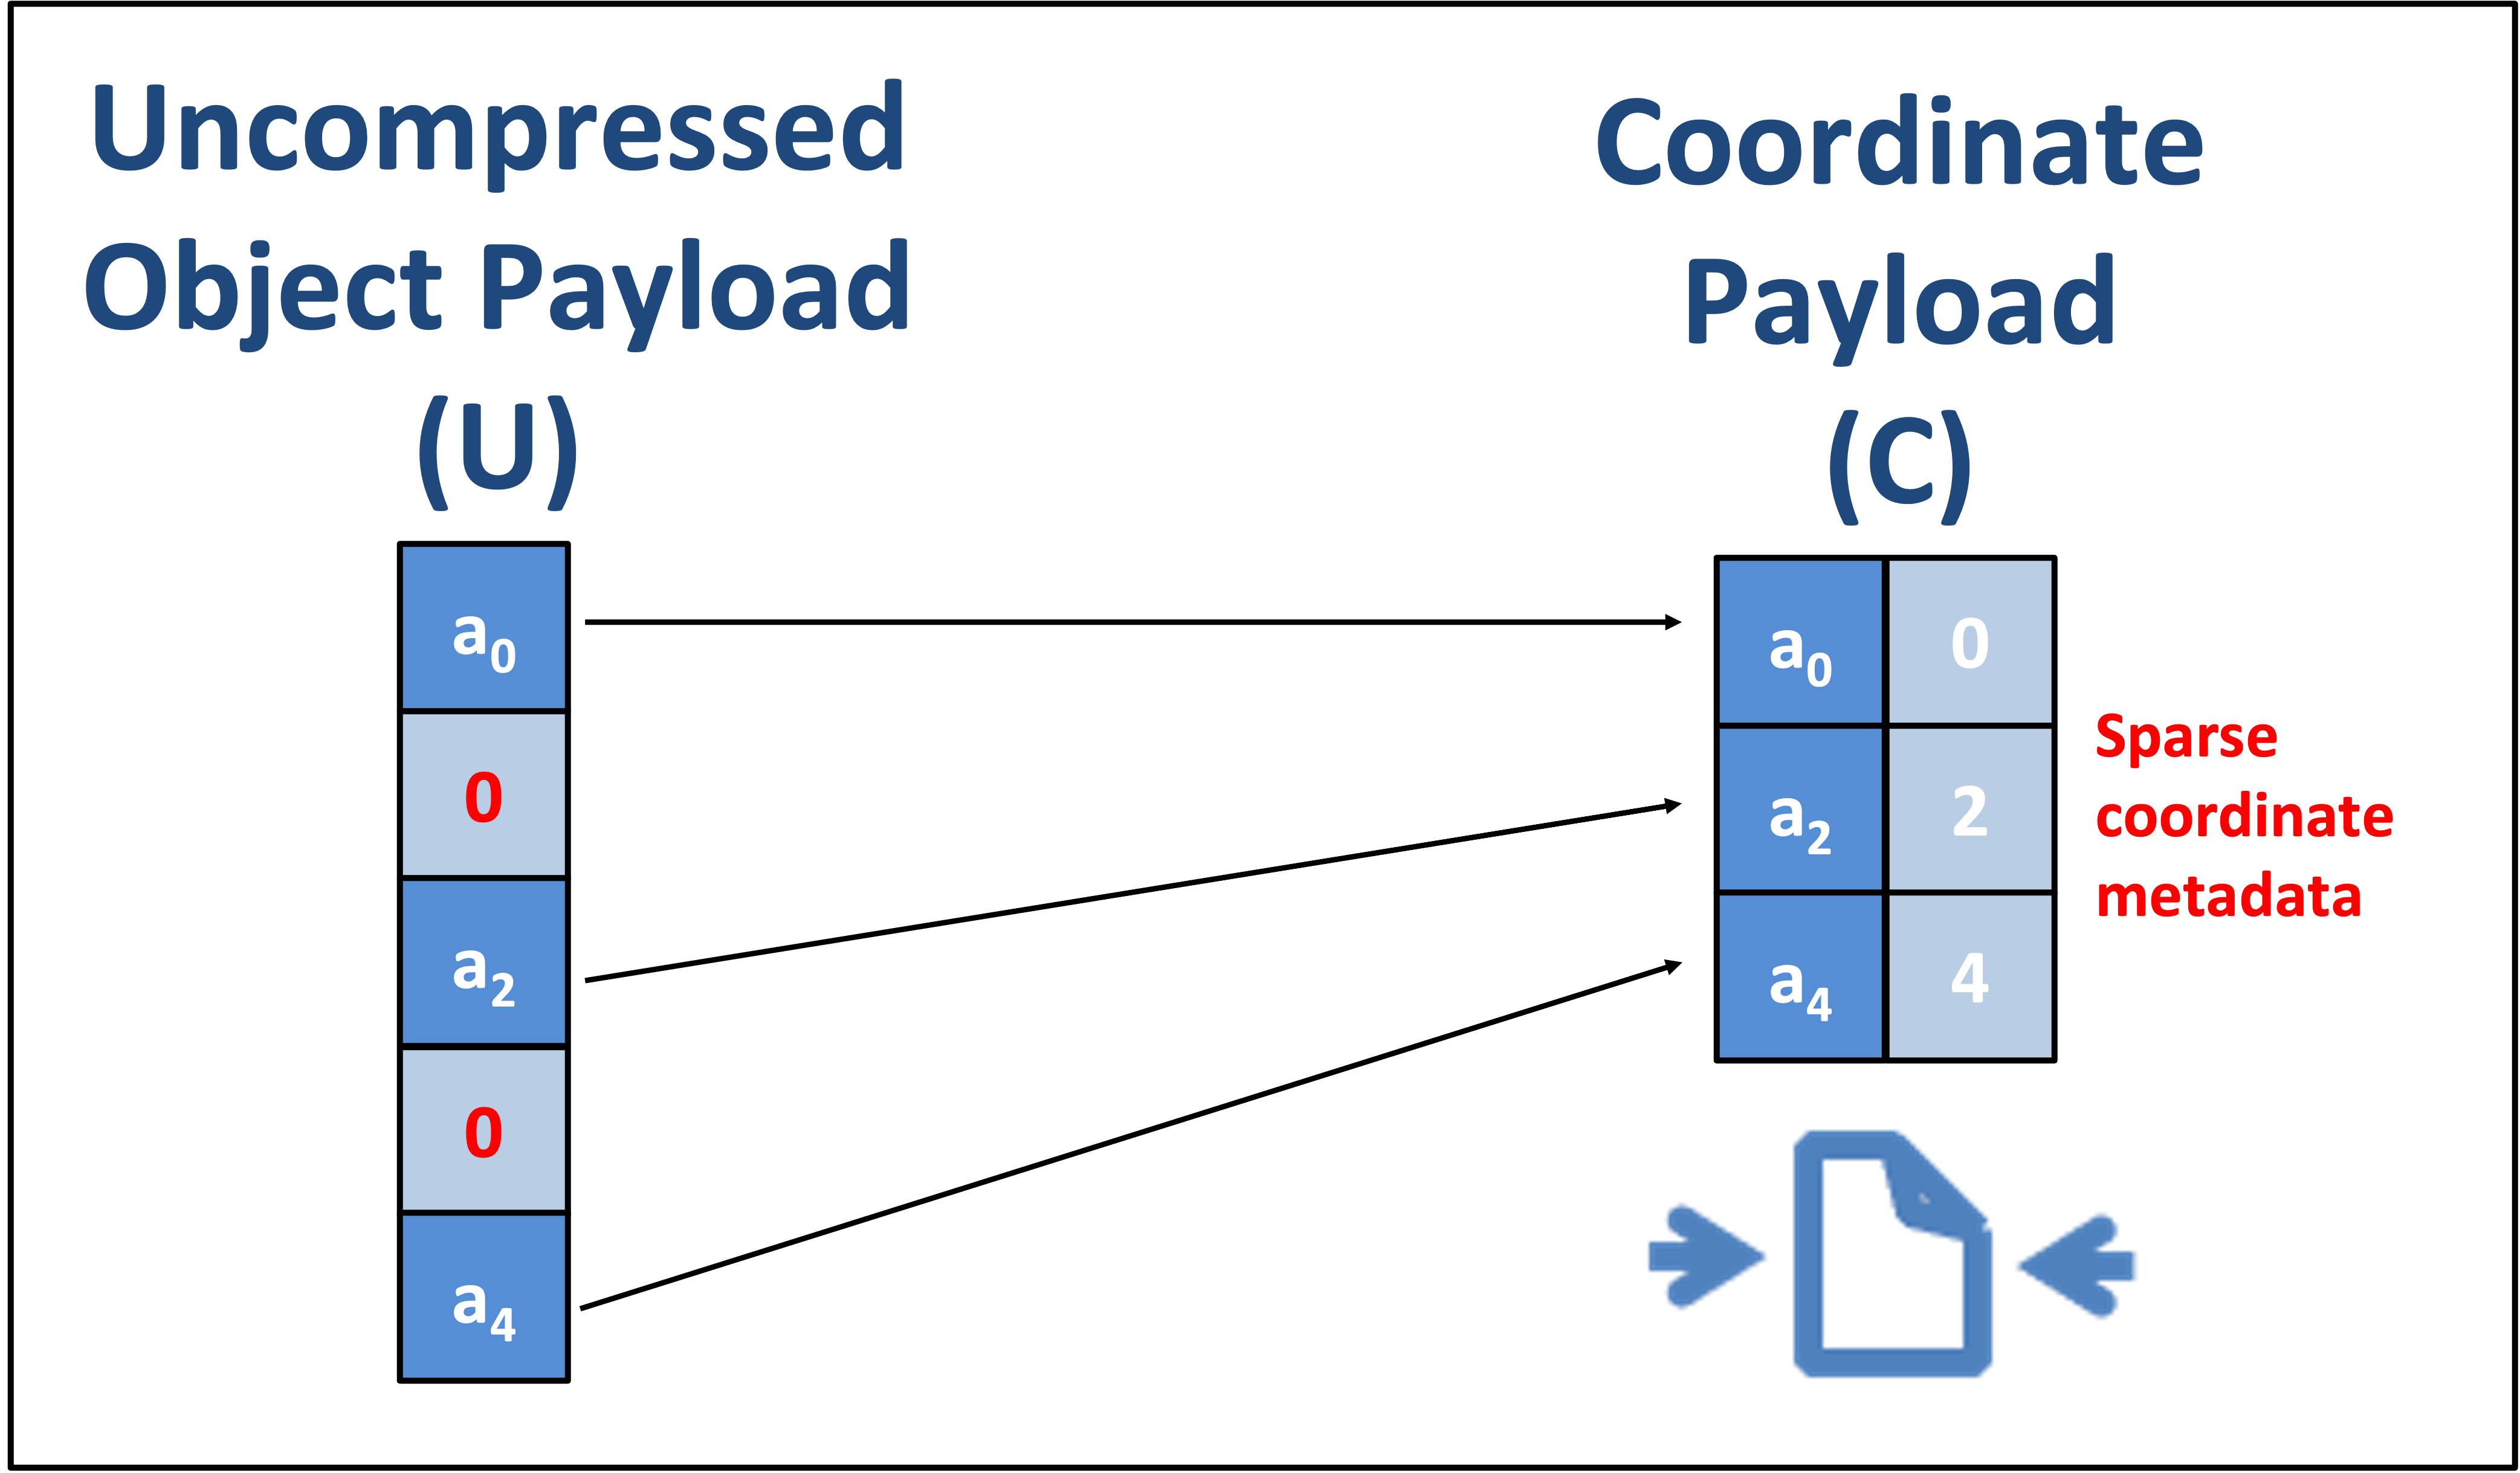
\includegraphics[width=8cm]{figures/saf_format_optimizations.PNG}
%\caption{A visualization of a compressed representation format (coordinate-payload or CP) applied to a vector with some zero entries. The compressed representation is reduced to nonzero values and metadata which recovers the original data structure.}
%\label{fig:saf_format_optimizations}
%\end{figure}
%
% Content: format optimizations
%

%
% Figure: combined action/format optimizations
%
%\begin{figure}[H]
%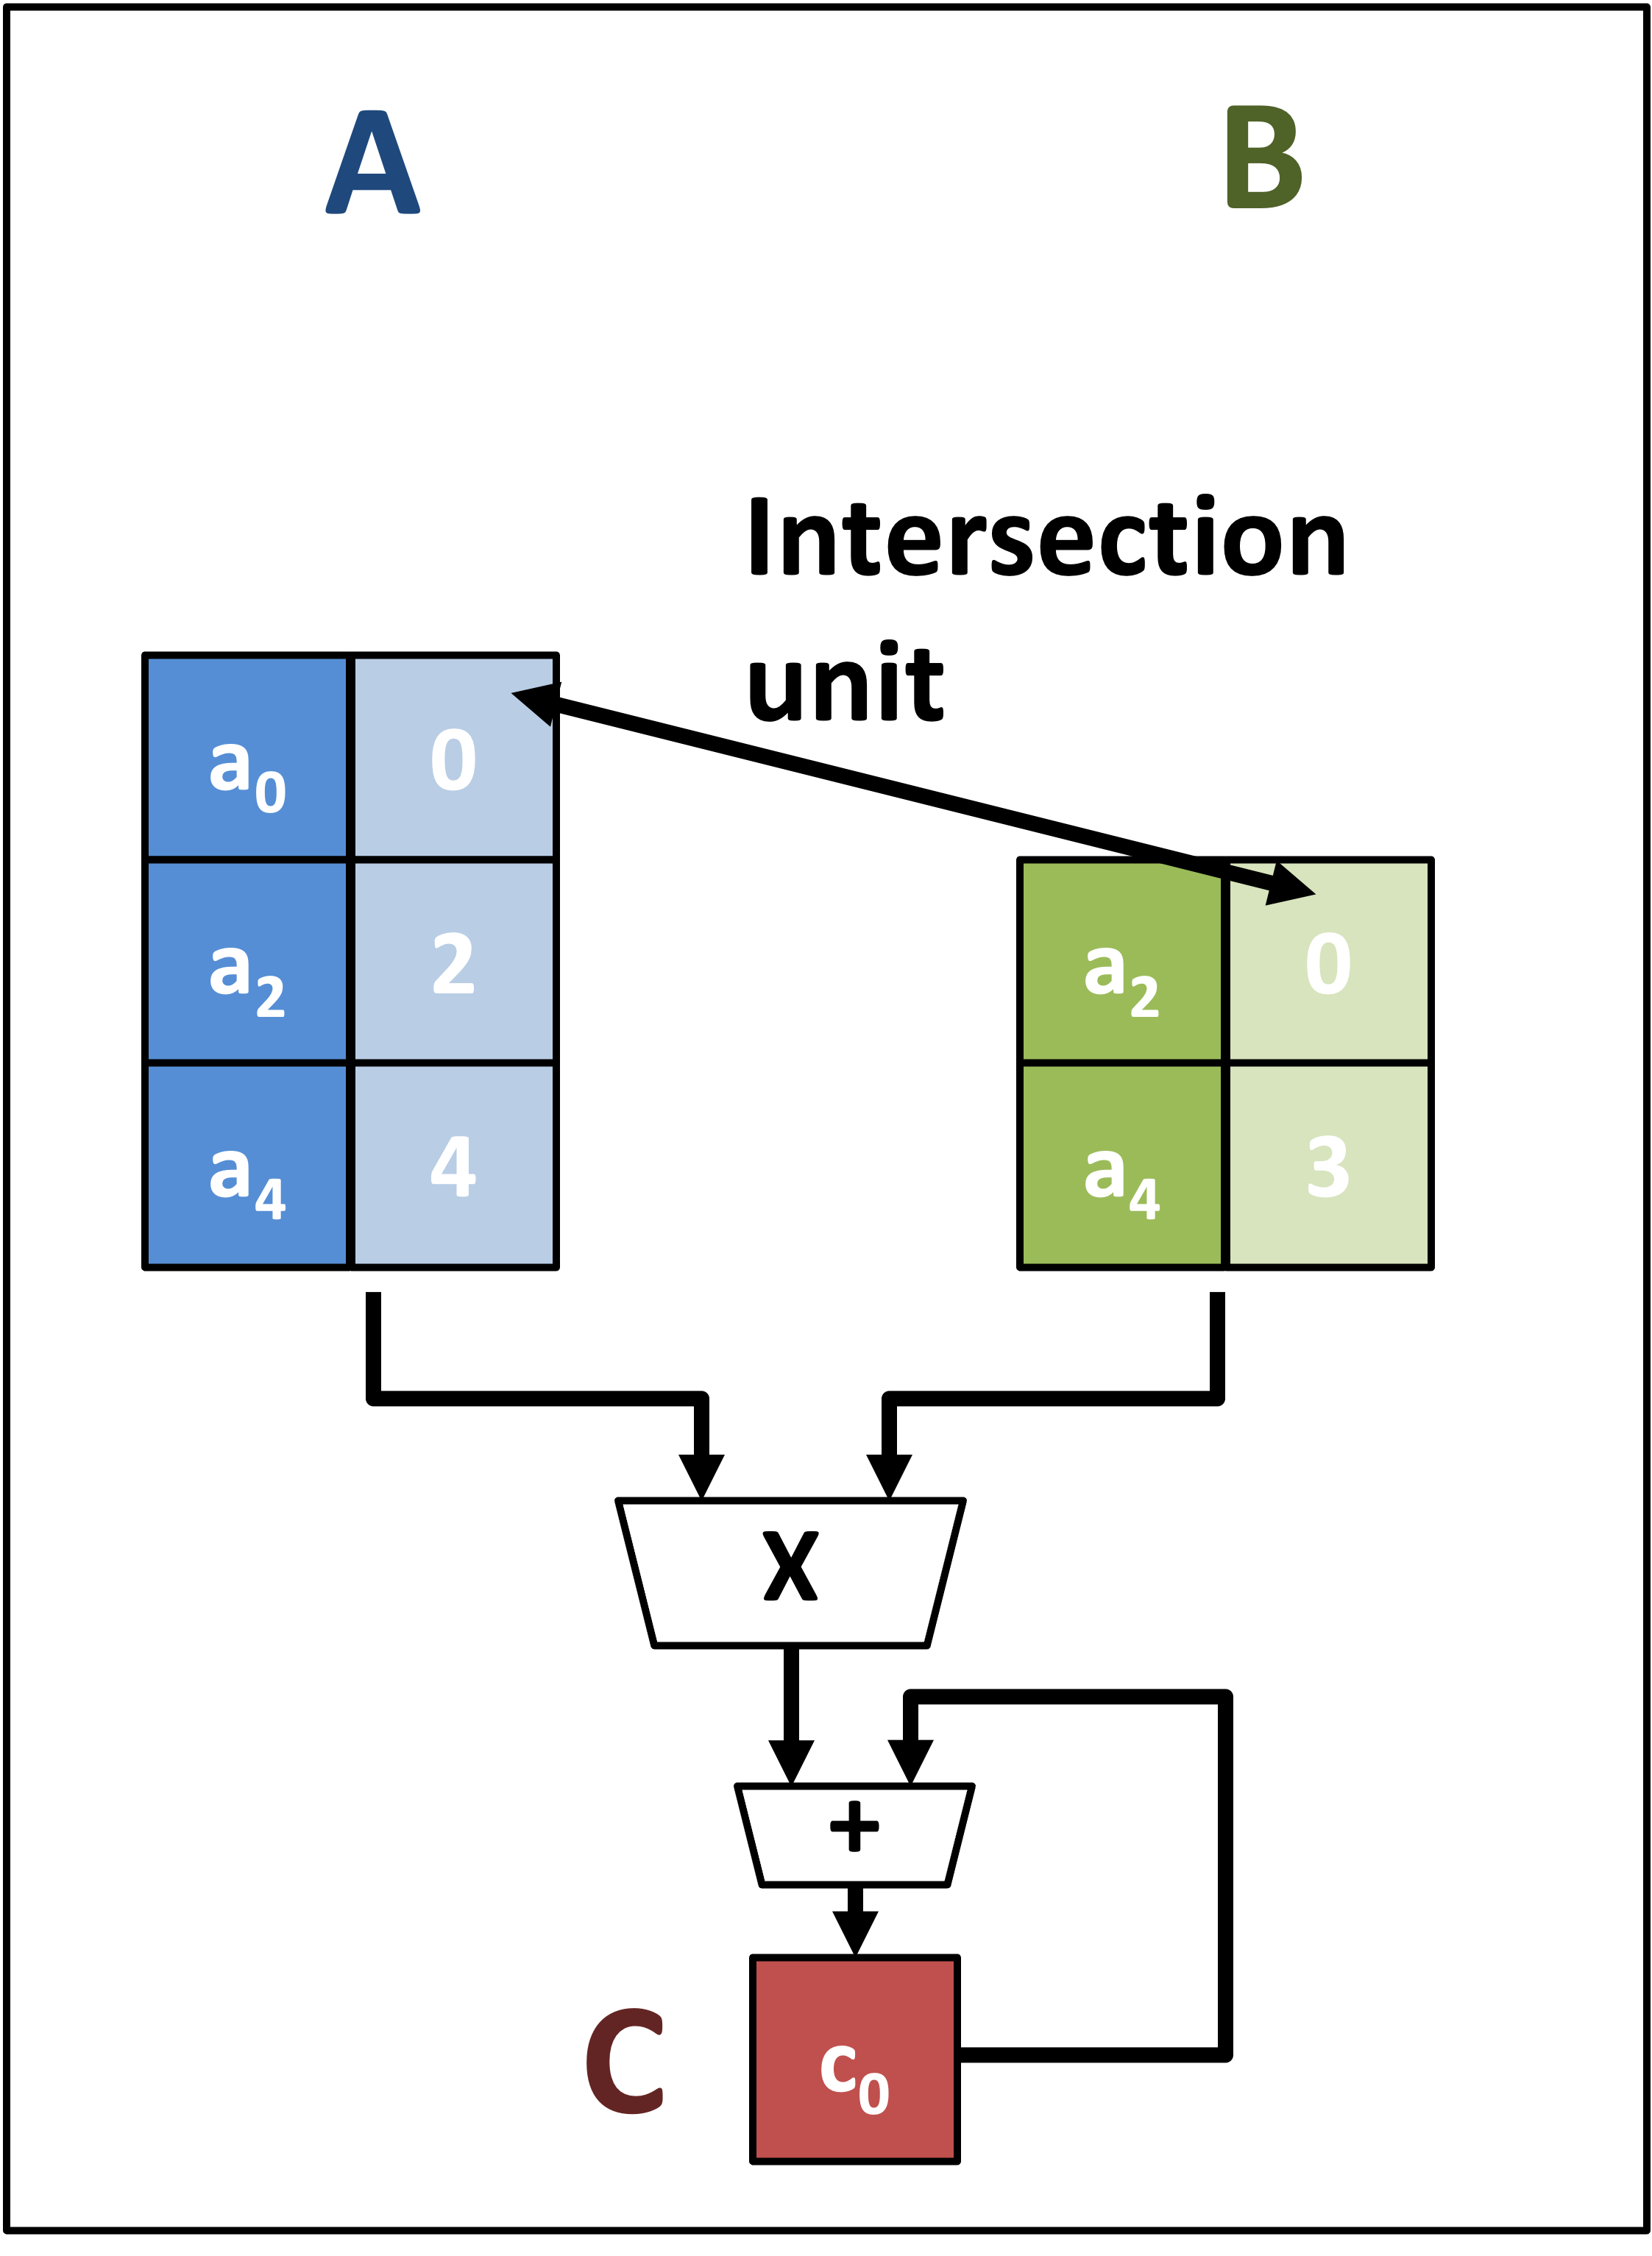
\includegraphics[width=4cm]{figures/saf_action_format_combo.PNG}
%\caption{An example of dot-product optimized with both bidirectional zero-skipping and a compressed representation format. Conceptually corresponding nonzero values must be matched using a component which processes format metadata in order to implement skipping, which is called an \textit{intersection unit.} The cost of the skipping optimization is the energy, area and latency of the skipping microarchitecture, which comprises the intersection unit.}
%\label{fig:saf_action_format_combo}
%\centering
%\end{figure}

%\subsubsection{Sparseloop workflow}

%\begin{figure}[H]
%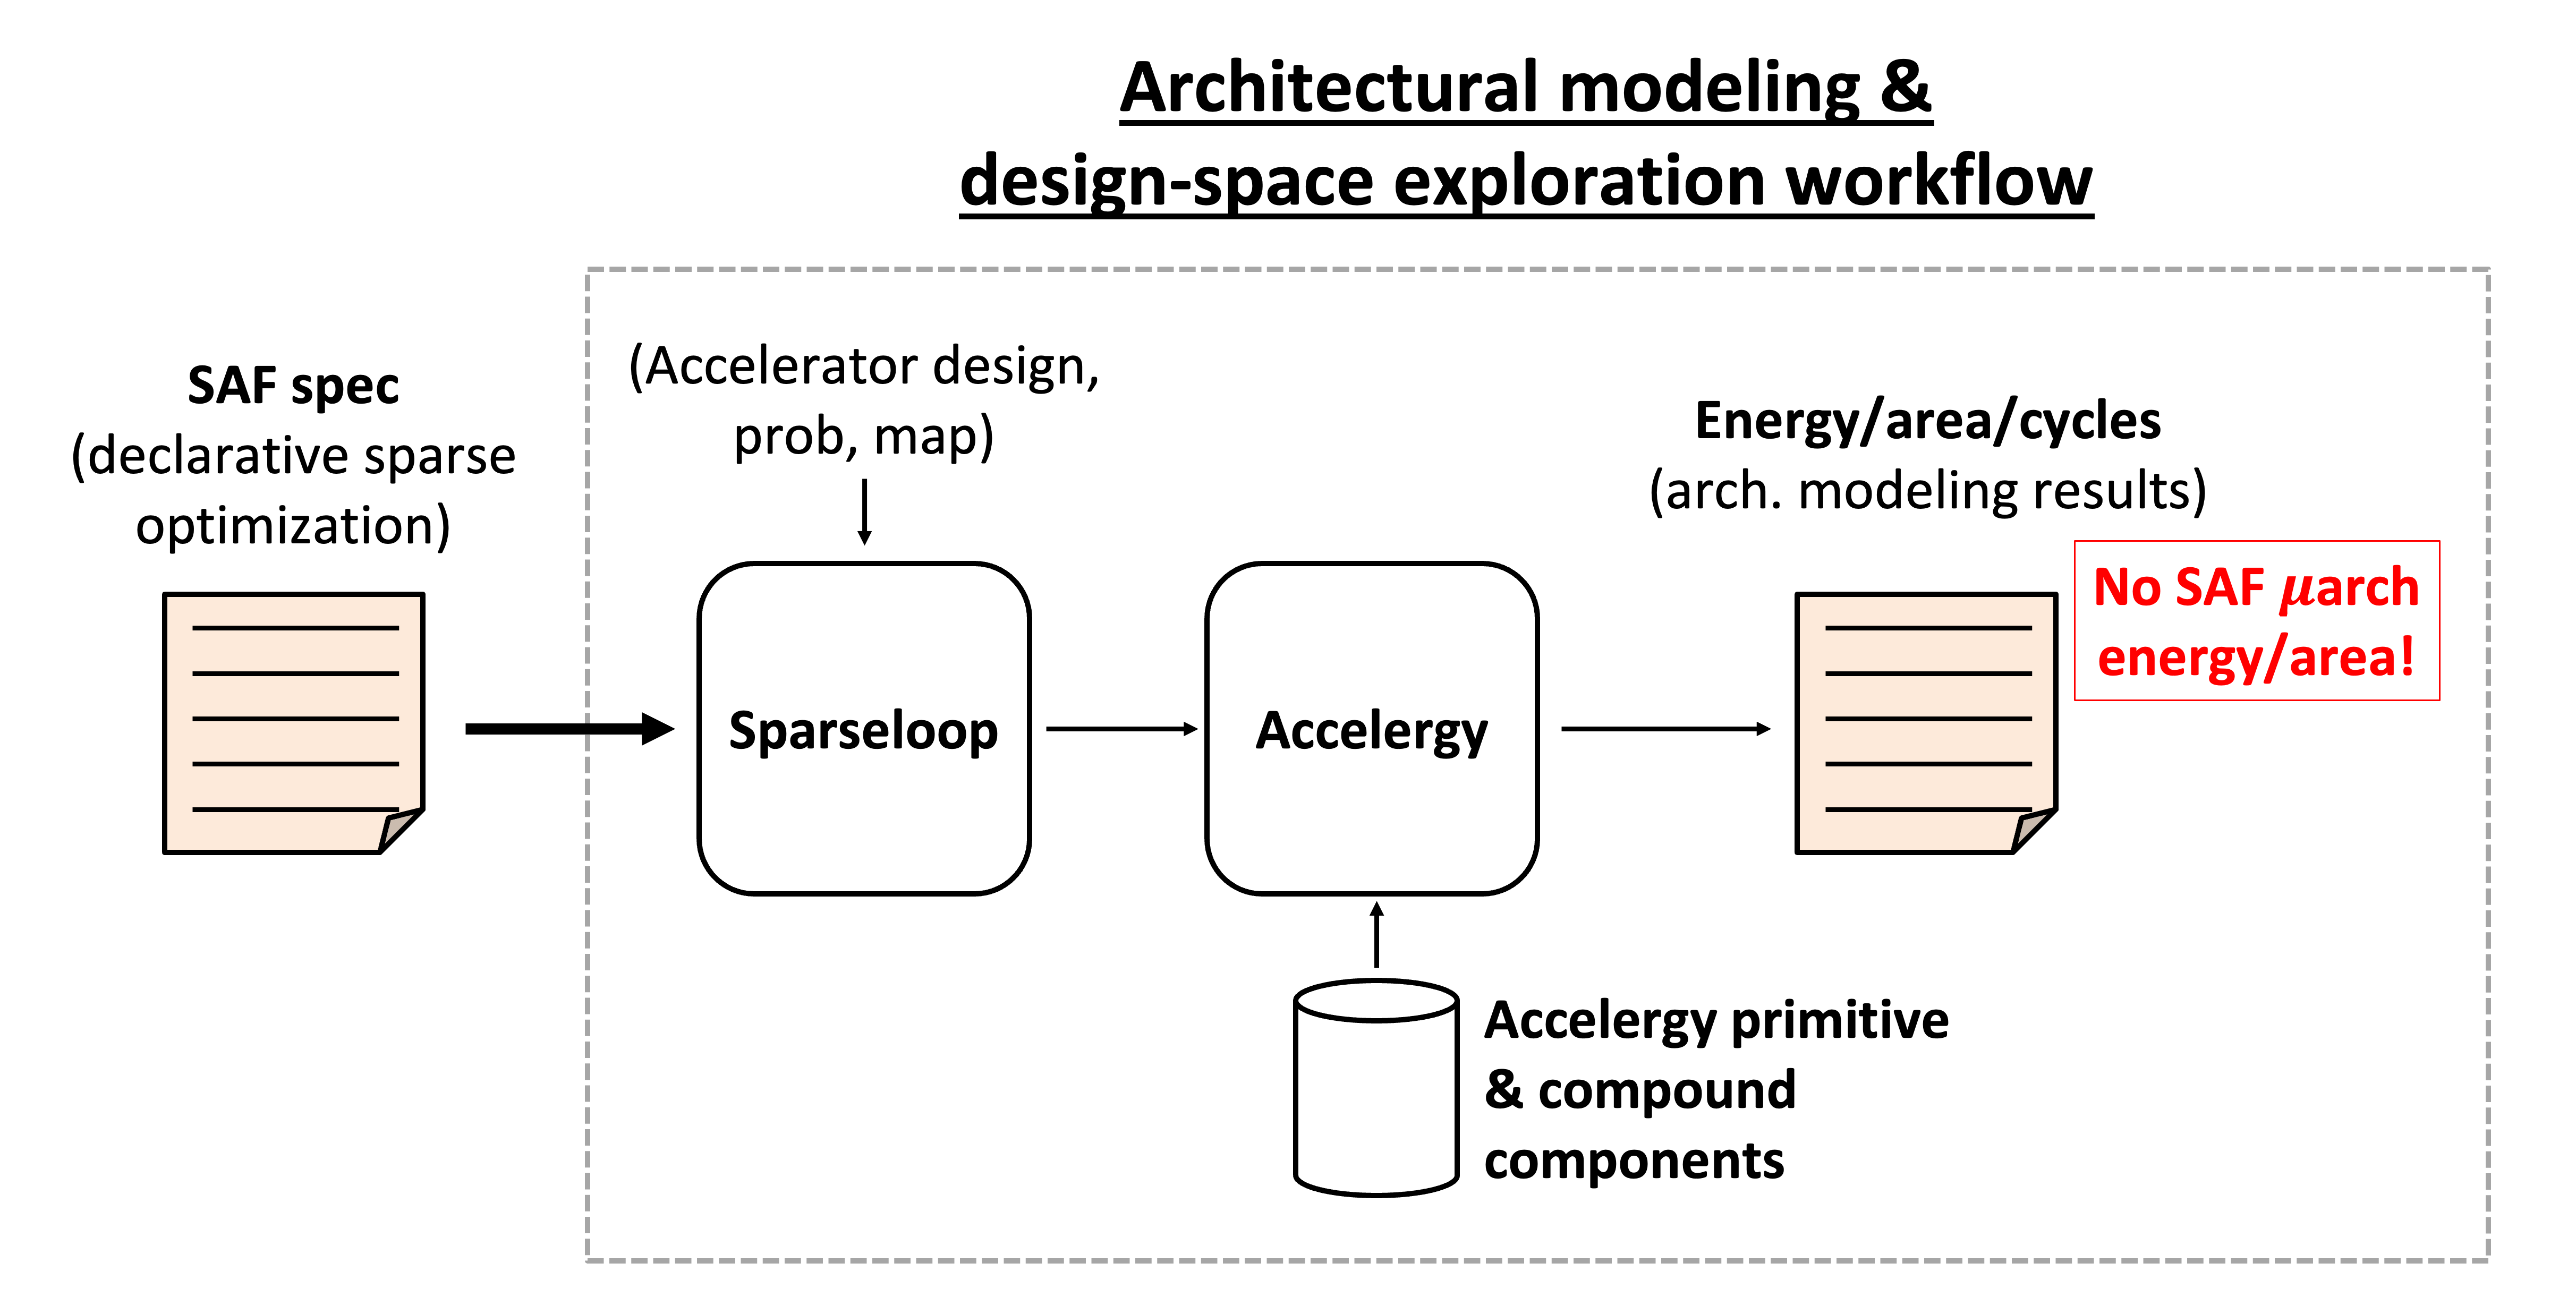
\includegraphics[width=8cm]{figures/sparseloop_workflow.png}
%\caption{The Sparseloop workflow for architectural modeling and %design-space exploration, simplified.}
%\label{fig:sparseloop_workflow}
%\end{figure}

\section{SAF microarchitectures}
\label{background:saf_uarch}
%
% Figure: SAFs can be significant or not, it depends on the microarchitecture
%
\begin{figure}[H]
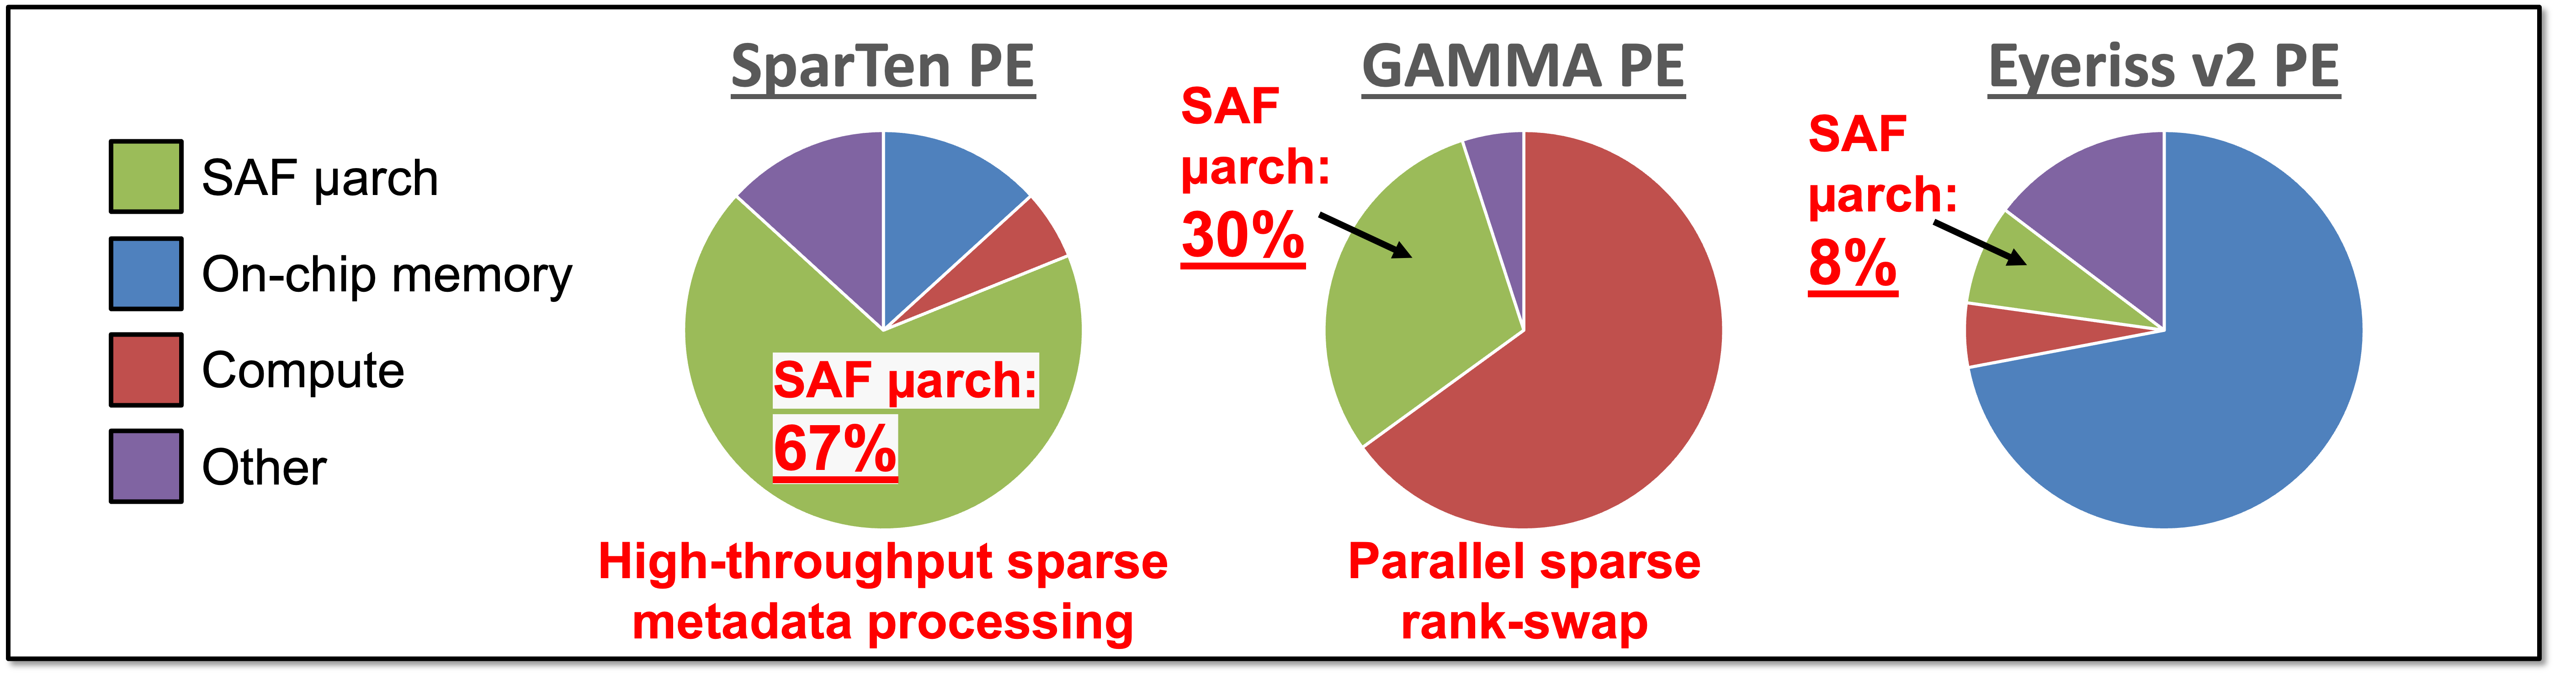
\includegraphics[width=\textwidth]{figures/saf_uarch_significance.PNG}
\caption{Breakdown of sparse tensor accelerator PE area based on published RTL simulations for a representative sample of designs. The total area of PE architectural components is a decent model of Eyeriss v2\cite{eyerissv2} PE area because Eyeriss v2's simple leader-follower zero-skipping microarchitecture has negligible area. SparTen\cite{sparten} employs a complex zero-skipping microarchitecture which must process high-throughput bitmask metadata. GAMMA's\cite{gamma} PE coordinates loop-nest re-ordering with tensor layout shuffling while the data is in-flight, using a high-radix merger component. These complex microarchitectures create discrepancies against architectural PE models.}
\label{fig:saf_uarch_significance}
\centering
\end{figure}

Prior research on sparse tensor acclerators proposes many different SAF microarchitectures, without employing a consistent set of abstractions and models in order to explore the design space or make comparisons. However, the breakdown of PE area for several accelerator designs in Figure~\ref{fig:saf_uarch_significance} shows that it is not always safe to assume SAF microarchitecture overhead is insignificant, and so it is important to choose SAFs and SAF microarchitecture designs systematically to minimize cost.

The Eyeriss v2\cite{eyerissv2} PE implements a leader-follower skipping SAF, devoting only 8\% of its PE area to the skipping microarchitecture. This is owing to a lightweight leader-follower skipping microarchitecture which operates on sparse weights and activations in Compressed-Sparse Column (CSC) format. 

In contrast, most of the area of the SparTen\cite{sparten} accelerator PE is devoted to the bidirectional skipping microarchitecture which operates on bitmask-format metadata.

As a final example, the GAMMA\cite{gamma} accelerator PE devotes 30\% of its PE area - a significant amount - in order to apply a rank swap\footnote{Rank swap refers to transposing tensor rank traversal order, as described in\cite{sparse_arch_lecture1}.}. 

Clearly, SAFs and SAF microarchitecture designs are complex and impactful design decisions, and it is desirable to know whether a particular combination of SAFs will lead to the substantial PE implementation overhead seen (for example) in SparTen and GAMMA. The rest of this work develops a conceptual framework for taxonomy and modeling of SAF microarchitectures. This conceptual framework can be represented in software and utilized to make SAF microarchitecture design decisions using analytical pre-RTL modeling tools.

%\subsection{Existing SAF microarchitecture designs}
%
%\begin{table}[h]
%\centering
%\resizebox{\textwidth}{!}{%
%\begin{tabular}{||l|l|l|l|l|l||}
%\hline
%\hline
%\textbf{Design} & \textbf{Workload} & \textbf{Sparse formats} & %\textbf{Action SAFs} & \textbf{$\mu$arch primitives} \\
%\hline
%\hline
%Eyeriss\cite{eyeriss} & DNN\cite{eyeriss}\cite{sparseloop} & \parbox[t]{5cm}{\cite{eyeriss}\cite{sparseloop}: \\ offchip: \\ - I/O: B-RLE \\ - W:U \\ onchip: \\ - I: UB \\ - O/W:U} & \parbox[t]{5cm}{\cite{eyeriss}\cite{sparseloop}: \\ Innermost storage: \\ - Gate W $<$- I \\ - Gate O $<$- I} & RLE (de)comp.\cite{eyeriss} \\
%\hline
%SparTen\cite{sparten} & DNN\cite{sparten} & - B (PE)\cite{sparten} & Skip (BD) (PE)\cite{sparten} & \parbox[t]{5cm}{\cite{sparten}: \\ B isect. \\ Pref.-sum (B$->$pos) \\ Pri.-enc. (compaction)} \\
%\hline
%Eyeriss v2\cite{eyerissv2} & DNN\cite{sparseloop}\cite{eyerissv2} & \parbox[t]{5cm}{\cite{eyerissv2}\cite{sparseloop}: \\ - I/W: B-UOP-CP (B-CSC) \\ - O:U} & \parbox[t]{5cm}{\cite{eyerissv2}: \\ Innermost storage: \\ - Skip W $<$- I \\ - Skip O $<$- I \& W \\ - Gate Compute} & \\
%\hline
%Cambricon-X\cite{cambricon_x} & DNN\cite{cambricon_x} & & & \\
%\hline
%Cnvlutin\cite{cnvlutin} & DNN\cite{cnvlutin} & & & \\
%\hline
%EIE\cite{eie} & DNN\cite{eie} & & & \\
%\hline
%ExTensor\cite{extensor} & MM\cite{extensor}\cite{sparseloop} & \parbox[t]{5cm}{\cite{extensor} \\ - A/B: UOP-CPx5 \\ - Z: U} & \parbox[t]{5cm}{All Storage: \\ - Skip A$<->$B \\ - Skip Z$<->$A\&B} & - C isect. \\
%\hline
%MatRaptor\cite{matraptor} & MM\cite{matraptor}\cite{teaal} & - C$^2$SR\cite{matraptor} & Skip B $<$- A & Psum. merge \\
%\hline
%SIGMA\cite{sigma} & MM\cite{sigma}\cite{teaal} & \parbox[t]{5cm}{B} & & \\
%\hline
%SpArch\cite{sparch} & MM\cite{sparch}\cite{teaal} & & & Parallel merge\cite{sparch} \\
%\hline
%Tensaurus\cite{tensaurus} & Some einsums\cite{tensaurus}\cite{teaal} & & & \\
%\hline
%GAMMA\cite{gamma} & MM\cite{gamma}\cite{teaal} & \parbox[t]{5cm}{\cite{gamma}: \\ - A: CSR \\ - B: CSR}  & \parbox[t]{5cm}{Skip B $<$- A} & \parbox[t]{5cm}{- Transp. merge-and-sum \\ - Fiber fetcher \\ - Leader val. LUT \\ } \\
%\hline
%\hline
%\end{tabular}%
%}
%\caption{Summary of Designs}
%\end{table}

%\begin{table}[h]
%\centering
%\resizebox{\textwidth}{!}{%
%\begin{tabular}{||l|l|l|l|l|l||}
%\hline
%\hline
%\textbf{Design} & \textbf{Workload} & \textbf{Sparse %formats} & \textbf{Action SAFs} & \textbf{$\mu$arch primitives} \\
%\hline
%\hline
%Eyeriss\cite{eyeriss} & DNN\cite{eyeriss}\cite{sparseloop} & \parbox[t]{5cm}{\cite{eyeriss}\cite{sparseloop}: \\ offchip: \\ - I/O: B-RLE \\ - W:U \\ onchip: \\ - I: UB \\ %- O/W:U} & \parbox[t]{5cm}%{\cite{eyeriss}\cite{sparseloop}: \\ Innermost storage: \\ - Gate W $<$- I \\ - Gate O $<$- I} & RLE (de)comp.\cite{eyeriss} \\
%\hline
%SparTen\cite{sparten} & DNN\cite{sparten} & - B (PE)\cite{sparten} & Skip (BD) (PE)\cite{sparten} & \parbox[t]{5cm}{\cite{sparten}: \\ B isect. \\ Pref.-sum (B$->$pos) \\ Pri.-enc. (compaction)} \\
%\hline
%Eyeriss v2\cite{eyerissv2} & DNN\cite{sparseloop}\cite{eyerissv2} & \parbox[t]{5cm}{\cite{eyerissv2}\cite{sparseloop}: \\ - I/W: B-UOP-CP (B-CSC) \\ - O:U} & \parbox[t]{5cm}{\cite{eyerissv2}: \\ Innermost storage: \\ - Skip W $<$- I \\ - Skip O $<$- I \& W \\ - Gate Compute} & \\
%\hline
%Cambricon-X\cite{cambricon_x} & DNN\cite{cambricon_x} & & & \\
%\hline
%Cnvlutin\cite{cnvlutin} & DNN\cite{cnvlutin} & & & \\
%\hline
%EIE\cite{eie} & DNN\cite{eie} & & & \\
%\hline
%ExTensor\cite{extensor} & MM\cite{extensor}\cite{sparseloop} & \parbox[t]{5cm}{\cite{extensor} \\ - A/B: UOP-CPx5 \\ - Z: U} & \parbox[t]{5cm}{All Storage: \\ - Skip A$<->$B \\ - Skip Z$<->$A\&B} & - C isect. \\
%\hline
%MatRaptor\cite{matraptor} & MM\cite{matraptor}\cite{teaal} & - C$^2$SR\cite{matraptor} & Skip B $<$- A & Psum. merge \\
%\hline
%SIGMA\cite{sigma} & MM\cite{sigma}\cite{teaal} & \parbox[t]{5cm}{B} & & \\
%\hline
%SpArch\cite{sparch} & MM\cite{sparch}\cite{teaal} & & & Parallel merge\cite{sparch} \\
%\hline
%Tensaurus\cite{tensaurus} & Some einsums\cite{tensaurus}\cite{teaal} & & & \\
%\hline
%GAMMA\cite{gamma} & MM\cite{gamma}\cite{teaal} & \parbox[t]{5cm}{\cite{gamma}: \\ - A: CSR \\ - B: CSR}  & \parbox[t]{5cm}{Skip B $<$- A} & \parbox[t]{5cm}{- Transp. merge-and-sum \\ - Fiber fetcher \\ - Leader val. LUT \\ } \\
%\hline
%\hline
%\end{tabular}%
%}
%\caption{Summary of Designs}
%\end{table}


%
% Figure: prior work
%
%\begin{table}[ht]
%\begin{tabular}{c|c|}
%\textbf{Accelerator} & \textbf{SAF microarchitecture proposals} \\ \hline \hline
%Eyeriss &  MAC gating; in-flight RLE decompression \\ \hline
%Eyeriss v2 & CSC zero-skipping \\ \hline
%ExTensor & Hierarchical bidirectional zero-skipping \\ \hline
%SCNN & Memory conflict handling (binning output coordinates) \\ \hline
%SparTen & Bitmask zero-skipping, parallel compression, memory conflict handling \\ \hline
%OuterSPACE & Software rank-swap \\ \hline
%GAMMA & Leader-following intersection, hardware rank-swap \\ \hline
%\end{tabular}
%\caption{A non-exhaustive list of published tensor accelerators and their proposed SAF microarchitectures.}
%\label{tab:design_specific_models}
%\centering
%\end{table}

